%%    _____  _____
%%   |  __ \|  __ \    AUTHOR: Pedro Rivero
%%   | |__) | |__) |   ---------------------------------
%%   |  ___/|  _  /    DATE: November 10, 2021
%%   | |    | | \ \    ---------------------------------
%%   |_|    |_|  \_\   https://github.com/pedrorrivero
%%

\section{State preparation}

%% ----------------------------------------------------------------------------

\begin{frame}{Space parametrization and state preparation}

	Once we have ways of measuring our Hamiltonian, we need to be able to explore different quantum states; a process known as \textbf{state preparation}. This can be achieved by parametrizing the Hilbert/Fock space of states representing the system, and finding a way to prepare the corresponding quantum state in the processor given any combination of those parameters.

	\begin{multicols}{2}

		For this task we will be employing some of the IBM-Q quantum computers and simulators; accessible through the cloud via the \texttt{Qiskit} framework. Nevertheless, there is one major shortcoming: the dimension of the space at hand grows exponentially with the number of qubits $2N$ used in the representation of the system. This means that the parametrization will become too large to handle both in state of the art and forthcoming machines unless it is treated in a smart way.

		\columnbreak

		\begin{center}
			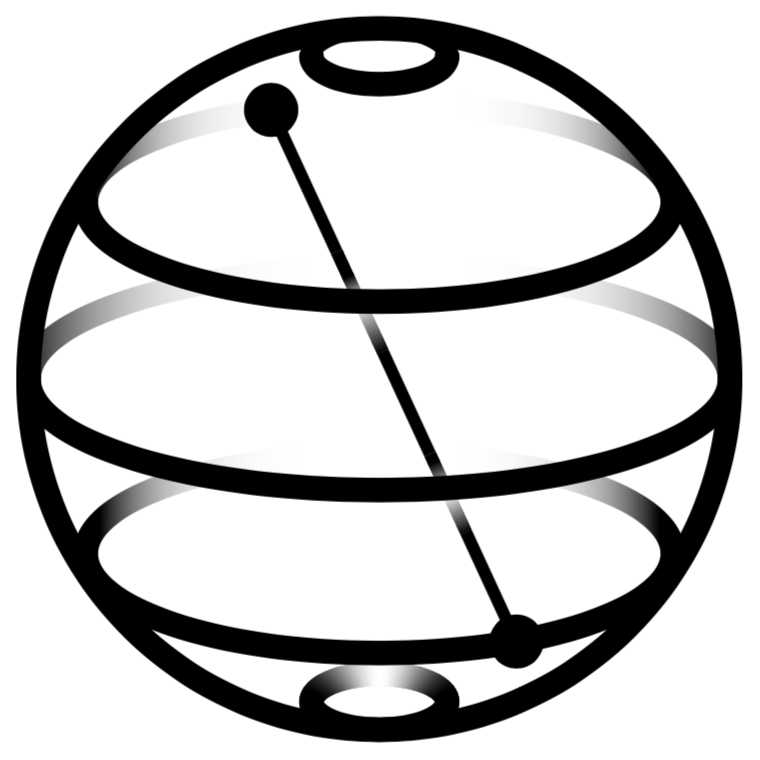
\includegraphics[width=.2\paperwidth]{Figures/qiskit}
		\end{center}
		\begin{center}
			
\includegraphics[width=.1\paperwidth]{Figures/ibm}
		\end{center}

	\end{multicols}

\end{frame}

%% ----------------------------------------------------------------------------

\begin{frame}[allowframebreaks]{Custom symmetry-based parametrization ansatz}

	While general, it is easy to notice that the implementation of any variant of the unitary coupled cluster ansatz is still cumbersome and can depend on a large number of parameters based on the chosen order of truncation. We will now introduce a new ansatz inspired by the shape of our refactored Hamiltonian. For this task, we will analyze the two distinct parts in our Hamiltonian independently; since these will dominate in two \textbf{different regimes}:

	\begin{multicols}{2}

		\begin{center}
			\underline{\textbf{INFINITELY STRONG INTERACTIONS}}\\
			\small{\emph{Interaction term dominates (i.e. $G_{\pi} \ra \infty$)}}
			\begin{gather*}
				G_{N} \defeq \sum_{n=0}^{N-1} Z_{2n+1}Z_{2n}
			\end{gather*}
		\end{center}

		\columnbreak

		\begin{center}
			\underline{\textbf{INFINITELY WEAK INTERACTIONS}}\\
			\small{\emph{Kinetic term dominates (i.e. $G_{\pi} \ra 0$)}}
			\begin{gather*}
			  K_{N} \defeq \sum_{n=0}^{2N-1} \qty[ X_{n+1}Y_{n} - Y_{n+1}X_{n} ]
			\end{gather*}
		\end{center}

	\end{multicols}

	Let us call each computational basis state by the decimal translation of its binary form:

	\begin{gather*}
	  \ket{0} \defeq \ket{\bin\dots0000} \qc
	  \ket{1} \defeq \ket{\bin\dots0001} \qc
	  \ket{2} \defeq \ket{\bin\dots0010} \qc
	  \cdots
	\end{gather*}

%% ----------------------------------------------------------------------------
\break
%% ----------------------------------------------------------------------------

	For the \textbf{interaction term} we notice that:

	\medskip

	\begin{itemize}
	  \item We can cycle in steps of two computational lattice sites.
	  \item We can change the position of any theoretical lattice site; since the interaction only occurs between positive and negative energy components at the same spot.
	  \item We can interchange positive and negative components in any number of theoretical lattice sites. We call each of these a \emph{swap transformation}.
	  \item We can flip every component $0 \lra 1$ in any number of theoretical lattice sites. We call each of these a \emph{flip transformation}.
	\end{itemize}

	\medskip

	This means that for $N=2$ (i.e. $2^{2N}=16$ basis states):

	\begin{gather*}
	  \ket{0} \equiv \ket{3} \equiv \ket{12} \equiv \ket{15} \\
	  \ket{1} \equiv \ket{2} \equiv \ket{4} \equiv \ket{7} \equiv
	    \ket{8} \equiv \ket{11} \equiv \ket{13} \equiv \ket{14} \\
	  \ket{5} \equiv \ket{6} \equiv \ket{9} \equiv \ket{10}
	\end{gather*}

%% ----------------------------------------------------------------------------
\break
%% ----------------------------------------------------------------------------

	Which represent the partition in degenerate subspaces of associated eigenvalues $\qty{+2,0,-2}$ respectively. These eigenvalues come from each theoretical lattice site in the spin-Z basis contributing with either $\pm 1$. Notice that the eigenvalues of this operator are always symmetrically disposed about zero, which means that $\forall N$:

	\begin{gather*}
	  \gamma_{\text{max}}^{N} = - \gamma_{\text{min}}^{N}
	\end{gather*}

	The interaction is maximum inside any theoretical lattice site whenever there is equal presence of both positive and negative energy components; conversely, the interaction is minimum whenever there is only one component present. Of course, the maximum (minimum) of the operator occurs when all theoretical lattice sites are maximized (minimized) individually:

	\begin{gather*}
	  \ket{\gamma_{\text{max}}}_{n} \in \{\ket{\bin00}, \ket{\bin11}\} \qc
	  \ket{\gamma_{\text{min}}}_{n} \in \{\ket{\bin01}, \ket{\bin10}\} \\[5pt]
	  \ket{\gamma_{\text{max}}^{N}} \equiv
	    \ket{\gamma_{\text{max}}}^{\otimes N} \qc
	  \ket{\gamma_{\text{min}}^{N}} \equiv
	    \ket{\gamma_{\text{min}}}^{\otimes N}
	\end{gather*}

%% ----------------------------------------------------------------------------
\break
%% ----------------------------------------------------------------------------

	Moving on to the \textbf{kinetic term} we have:

	\medskip

	\begin{itemize}
	  \item We can cycle in steps of one computational lattice site. We call this a \emph{cycling transformation}.
	  \item We cannot change the position of any theoretical lattice site; since the computational lattice sites now form a chain with their nearest neighbors.
	  \item If we interchange positive and negative components in all theoretical lattice sites, the resulting expectation value flips its sign (i.e. \emph{global swap transformations} are antisymmetric).
	  \item Flip transformations do not represent any apparent symmetry.
	\end{itemize}

	\medskip

	Once more, this operator has its eigenstates symmetrically disposed around zero. Also, global swap transformations are equivalent to complex conjugation:

	\begin{gather*}
		\kappa_{\text{max}}^{N} = -\kappa_{\text{min}}^{N} \\
		K_{N}^{\dagger} = \qty(K_{N}^{*})^{T} = \qty(-K_{N})^{T} = K_{N} \qRa
	    K_{N}^{T} = -K_{N} = K_{N}^{*}
	\end{gather*}

%% ----------------------------------------------------------------------------
\break
%% ----------------------------------------------------------------------------

	\begin{table}[!bp]
	  \centering
	  \caption{Global swap transformations for the $N=2$ basis states according to their number of particles.}
	  \label{tab:symmetry-ansatz-basis2-swaps}
	  \begin{tabular}{ c l }
	    \hline
	    % \rule{0pt}{14pt}
	    $N_\text{particles}$ & Global swap transformations \\
	    \hline
	    \hline
	    % \rule{0pt}{14pt}
	    $0$ & $\ket{0} \lra \ket{0}$ \\
	    \hline
	    $1$ & $\ket{1} \lra \ket{2} \qc \ket{4} \lra \ket{8}$ \\
	    \hline
	    $2$ & $\ket{3} \lra \ket{3} \qc \ket{5} \lra \ket{10} \qc
	      \ket{6} \lra \ket{9} \qc \ket{12} \lra \ket{12}$ \\
	    \hline
	    $3$ & $\ket{7} \lra \ket{11} \qc \ket{13} \lra \ket{14}$ \\
	    \hline
	    $4$ & $\ket{15} \lra \ket{15}$ \\
	    \hline
	  \end{tabular}
	\end{table}

	\begin{table}[!bp]
	  \centering
	  \caption{Cycles for the $N=2$ basis states according to their number of particles.}
	  \label{tab:symmetry-ansatz-basis2-cycles}
	  \begin{tabular}{ c l }
	    \hline
	    % \rule{0pt}{14pt}
	    $N_\text{particles}$ & Cycles \\
	    \hline
	    \hline
	    % \rule{0pt}{14pt}
	    $0$ & $\ket{0}$ \\
	    \hline
	    $1$ & $\ket{1} \lra \ket{2} \lra \ket{4} \lra \ket{8}$ \\
	    \hline
	    $2$ & $\ket{3} \lra \ket{6} \lra \ket{12} \lra \ket{9} \qc
	      \ket{5} \lra \ket{10}$ \\
	    \hline
	    $3$ & $\ket{7} \lra \ket{14} \lra \ket{13} \lra \ket{11}$ \\
	    \hline
	    $4$ & $\ket{15}$ \\
	    \hline
	  \end{tabular}
	\end{table}

%% ----------------------------------------------------------------------------
\break
%% ----------------------------------------------------------------------------

	If an eigenstate is not degenerate, it must comply with the rule that all amplitudes multiplying the states that make up its superposition, and which are related by a cycling transformation, must be the same up to a constant \emph{phase factor}:

	\begin{gather*}
	  e^{i\phi} \in
	    \qty{ \exp(i \frac{2\pi}{p} n) \qq{:} n \in \mathds{Z} \qq{and}
	    p \defeq \text{size of the smaller cycle} }
	\end{gather*}

	Finally, because this operator is made out of the Pauli X and Y matrices, and these matrices ---regardless of any phase factors--- flip the state they are applied to (i.e. $0 \lra 1$), we can see that any maximum (minimum) eigenstate will necessarily have the \textbf{same number of occupied and unoccupied states}. If we naively parametrize the space of states with this number of particles, we will get a prohibitive parametrization that grows exponentially in the number of basis states as $\binom{2N}{N}$. However, if we assume that these eigenstates are not degenerate, we can apply the above mentioned rules to build a simpler general form for them.

%% ----------------------------------------------------------------------------
\break
%% ----------------------------------------------------------------------------

	Because the smallest cycle for $N=2$ is of size two, any phase factors between elements of the same cycle can only be $\pm 1$. Also, we need to make sure that a swap transformation in all theoretical lattice sites ---equivalent to complex conjugation--- applied to the either the maximum or minimum eigenstate, reproduces its counterpart.

	\begin{gather*}
	  \alpha \frac{1}{\sqrt{2}} \qty(\ket{3}+\ket{12}) -
	  \beta \frac{1}{\sqrt{2}} \qty(\ket{6}+\ket{9})  +
	  \delta \frac{i}{\sqrt{2}} \qty(\ket{5} - \ket{10})
	\end{gather*}

	Which can then be converted into a general normalized form by resorting to an analogy with spherical coordinates. This results in the \textbf{symmetry based parametrization} (SBP):

	\begin{gather*}
	  \ket{\text{SBP}_{2} \qty(\theta, \eta)} \defeq
	    \sin(\theta)\sin(\eta) \ket{\gamma_{\text{max}}^2} -
	    \sin(\theta)\cos(\eta) \ket{\gamma_{\text{min},1}^2} + i
	    \cos(\theta) \ket{\gamma_{\text{min},2}^2} \\[5pt]
	  \ket{\gamma_{\text{max}}^2} \defeq
	    \frac{\ket{3}+\ket{12}}{\sqrt{2}} \qc
	  \ket{\gamma_{\text{min},1}^2} \defeq
	    \frac{\ket{6}+\ket{9}}{\sqrt{2}} \qc
	  \ket{\gamma_{\text{min},2}^2} \defeq
	    \frac{\ket{5} - \ket{10}}{\sqrt{2}}
	\end{gather*}

%% ----------------------------------------------------------------------------
\break
%% ----------------------------------------------------------------------------

	As a matter of fact, this state can indeed evaluate to the minimum and maximum eigenstates of the operator when $N=2$:

	\begin{gather*}
	  \ket{\kappa_{\text{max}}^{2}} =
	    \frac{1}{2\sqrt{2}} \qty(\ket{3}-\ket{6}-\ket{9}+\ket{12}) -
	    \frac{i}{2} \qty(\ket{5}-\ket{10}) \\
	  \ket{\kappa_{\text{min}}^{2}} =
	  \frac{1}{2\sqrt{2}} \qty(\ket{3}-\ket{6}-\ket{9}+\ket{12}) +
	  \frac{i}{2} \qty(\ket{5}-\ket{10})
	\end{gather*}

	The particular choice when assigning the basis states in the spherical coordinates analogy, was made so that these maximum and minimum eigenstates evaluate for simple values of the parameters:

	\begin{gather*}
	  \ket{\kappa_{\text{max}}^{2}} \equiv
	    \ket{\text{SBP}_{2} \qty(\frac{3\pi}{4}, \frac{\pi}{4})} \qc
	  \ket{\kappa_{\text{min}}^{2}} \equiv
	    \ket{\text{SBP}_{2} \qty(\frac{\pi}{4}, \frac{\pi}{4})} \\
	  \ket{\gamma_{\text{max}}^{2}} \equiv
	    \ket{\text{SBP}_{2} \qty(\frac{\pi}{2}, \frac{\pi}{2})} \qc
	  \ket{\gamma_{\text{min},1}^{2}} \equiv
	    \ket{\text{SBP}_{2} \qty(\frac{\pi}{2}, 0)} \qc
	  \ket{\gamma_{\text{min},2}^{2}} \equiv
	    \ket{\text{SBP}_{2} \qty(0, 0)}
	\end{gather*}

\end{frame}

%% ----------------------------------------------------------------------------

\begin{frame}[allowframebreaks]{Parametrization ansatz implementation}

	In order to implement this parametrization on any of the IBM-Q quantum computers, we need to be able to write it down as a quantum circuit. This means that it has to expressed through an unitary operator $U\qty(\theta, \eta)$ in the form:

	\begin{gather}
	  \ket{\text{SBP}_{2} \qty(\theta, \eta)} =
	    U\qty(\theta, \eta) \ket{\text{SR}}
	\end{gather}

	At first we will only be interested in obtaining the ground state energy of our system for positive values of the coupling constant (i.e. we will only need the minimum eigenstates), this allows us to simplify even further the parametrization introduced in the previous section. This will allow us to reduce the subspace we are looking into from three dimensions down to two.

	\begin{gather}
	  \ket{\gamma} \equiv
	    \ket{\gamma_{\text{min},2}^2} \defeq
	    \frac{\ket{5} - \ket{10}}{\sqrt{2}} \equiv
	    \ket{\text{SBP}_{2} \qty(0, \frac{\pi}{4})} \\
	  \ket{\kappa} \defeq
	    \frac{\ket{3}-\ket{6}-\ket{9}+\ket{12}}{2} \equiv
	    \ket{\text{SBP}_{2} \qty(\frac{\pi}{2}, \frac{\pi}{4})}
	\end{gather}

%% ----------------------------------------------------------------------------
\break
%% ----------------------------------------------------------------------------

	\begin{multicols}{2}

		This will effectively cut down the degrees of freedom from two to just one (i.e. fixing $\eta=\pi/4$). However, having now only two distinguishable quantum states, we can choose to ease the parametrization to account for the entirety of the Hilbert space associated to the \textbf{qubit} they comprise; spuriously increasing the degrees of freedom back to two, but making the implementation as a quantum circuit conceptually easier.

		\medskip

		We will parametrize an \textbf{ancilla qubit}, and then map its basis states to the two basis states of the subspace that we are interested in exploring.

		\columnbreak

		\begin{center}
			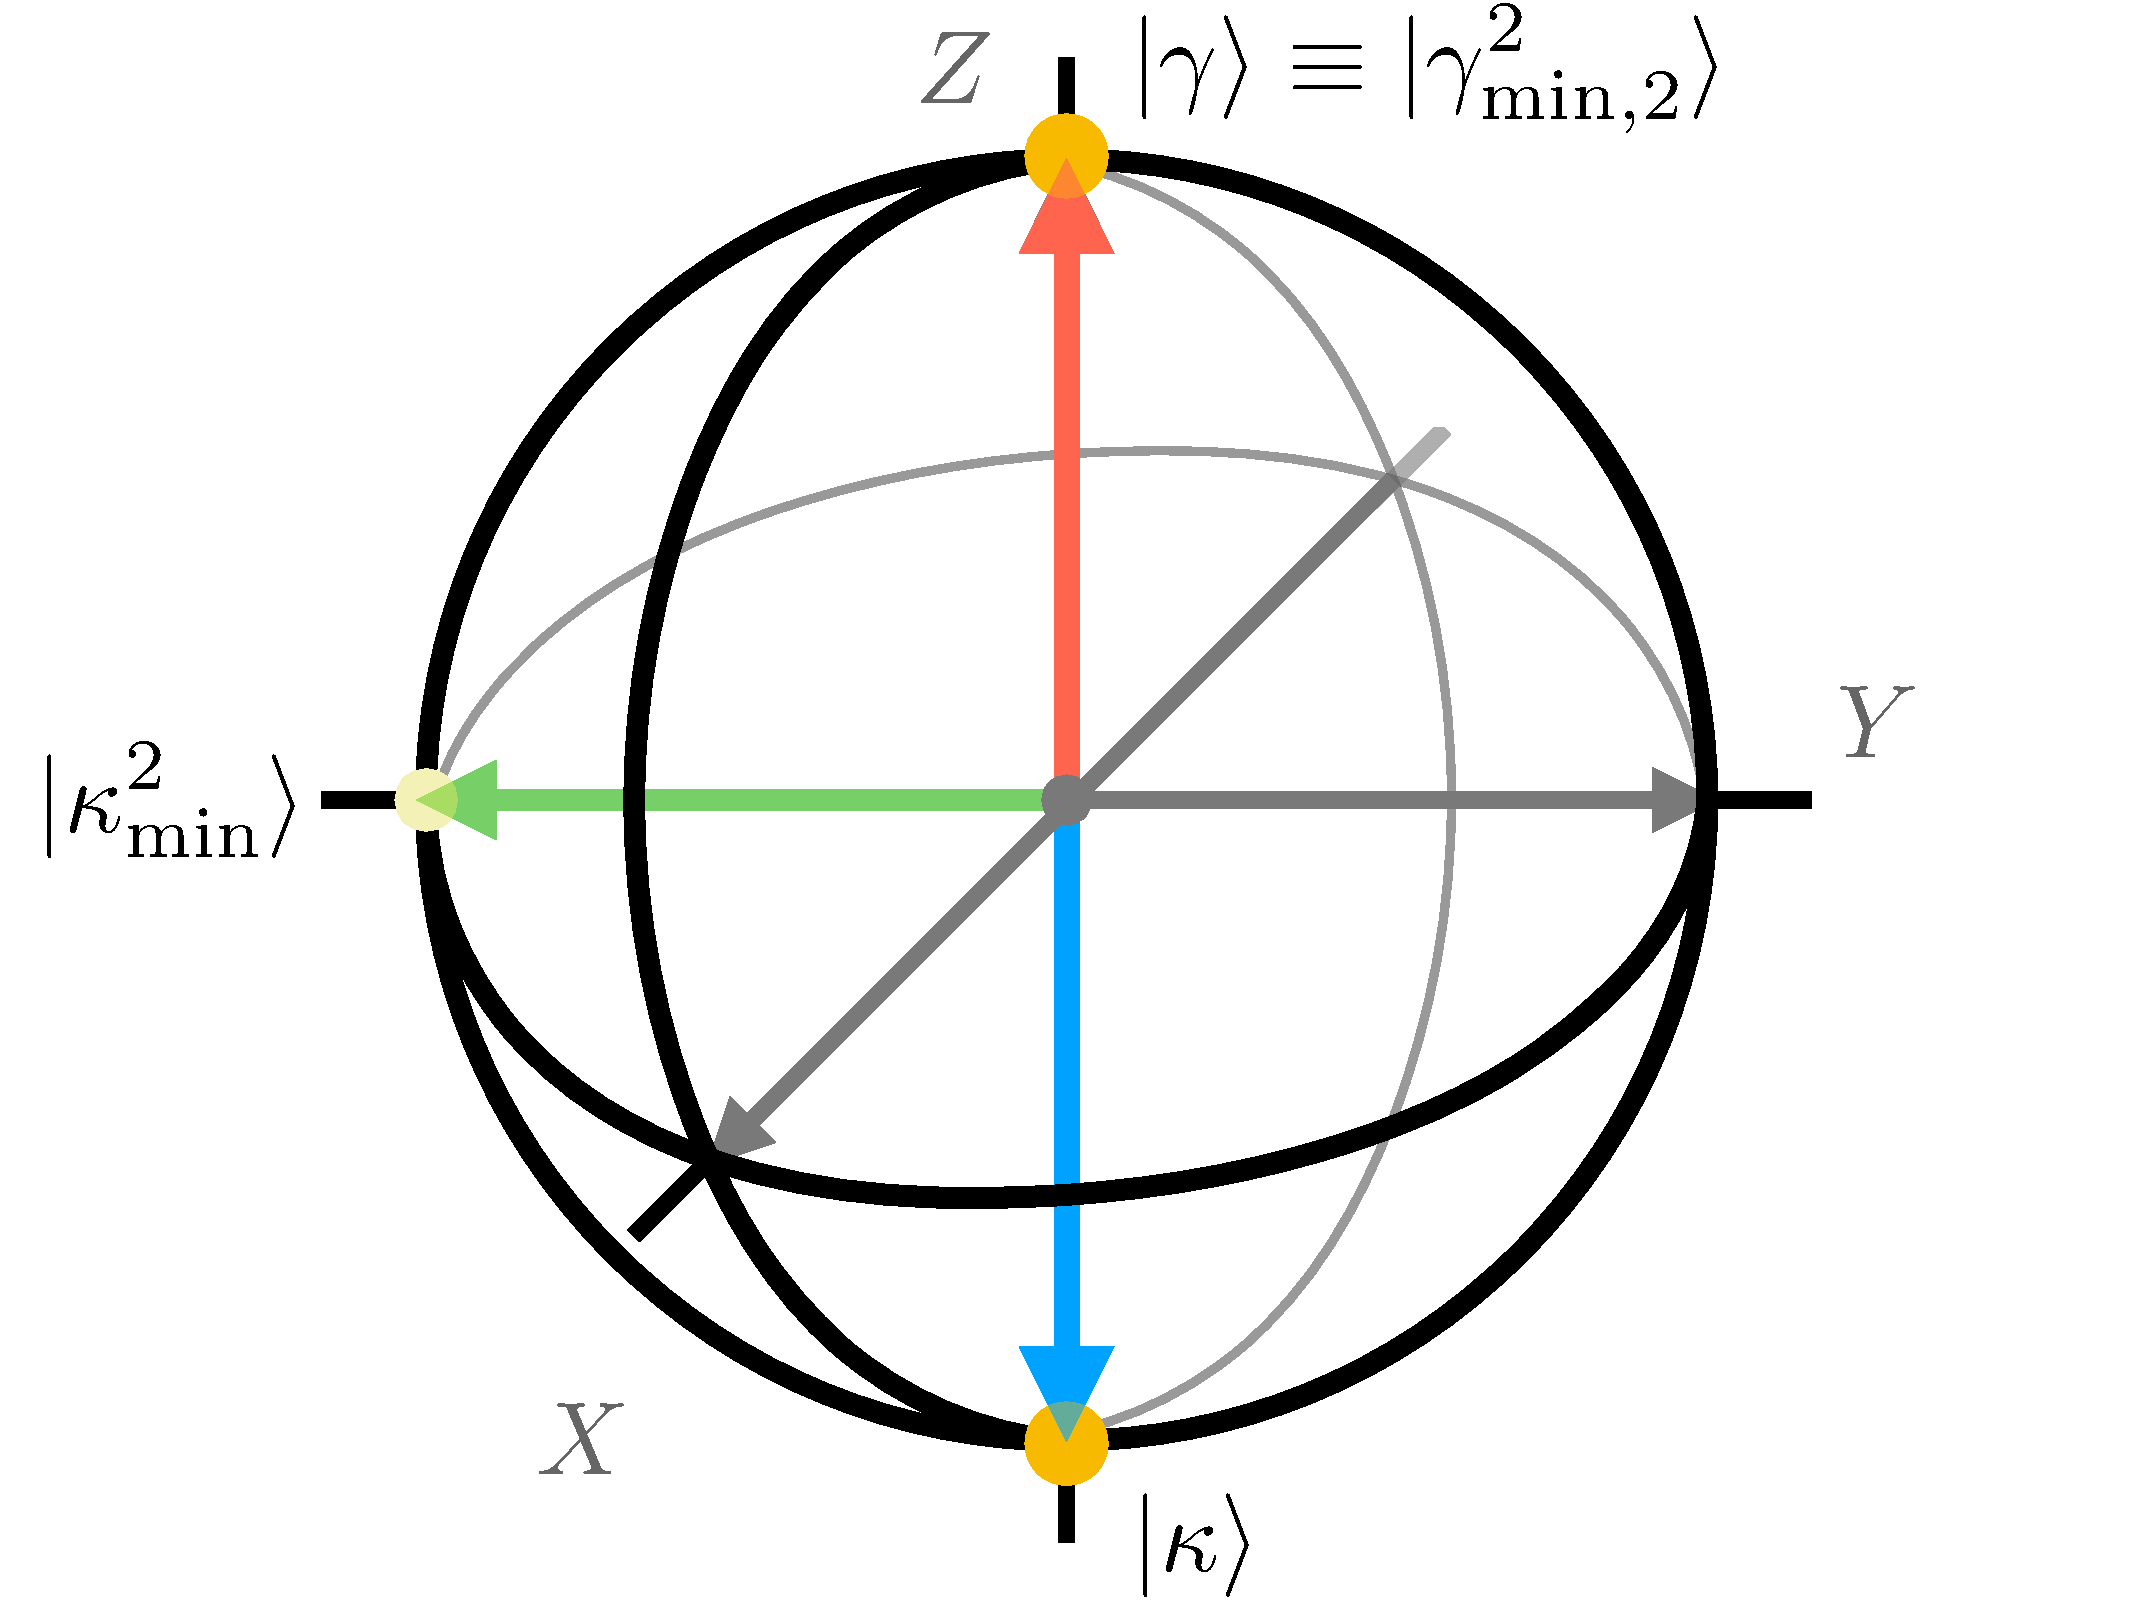
\includegraphics[width=.4\paperwidth]{Figures/NJL1-model-solving/bloch-sphere}
		\end{center}

	\end{multicols}

%% ----------------------------------------------------------------------------
\break
%% ----------------------------------------------------------------------------

	\begin{figure}[!p]
		\centering
		\begin{minipage}[c]{.45\linewidth}
			\centering
			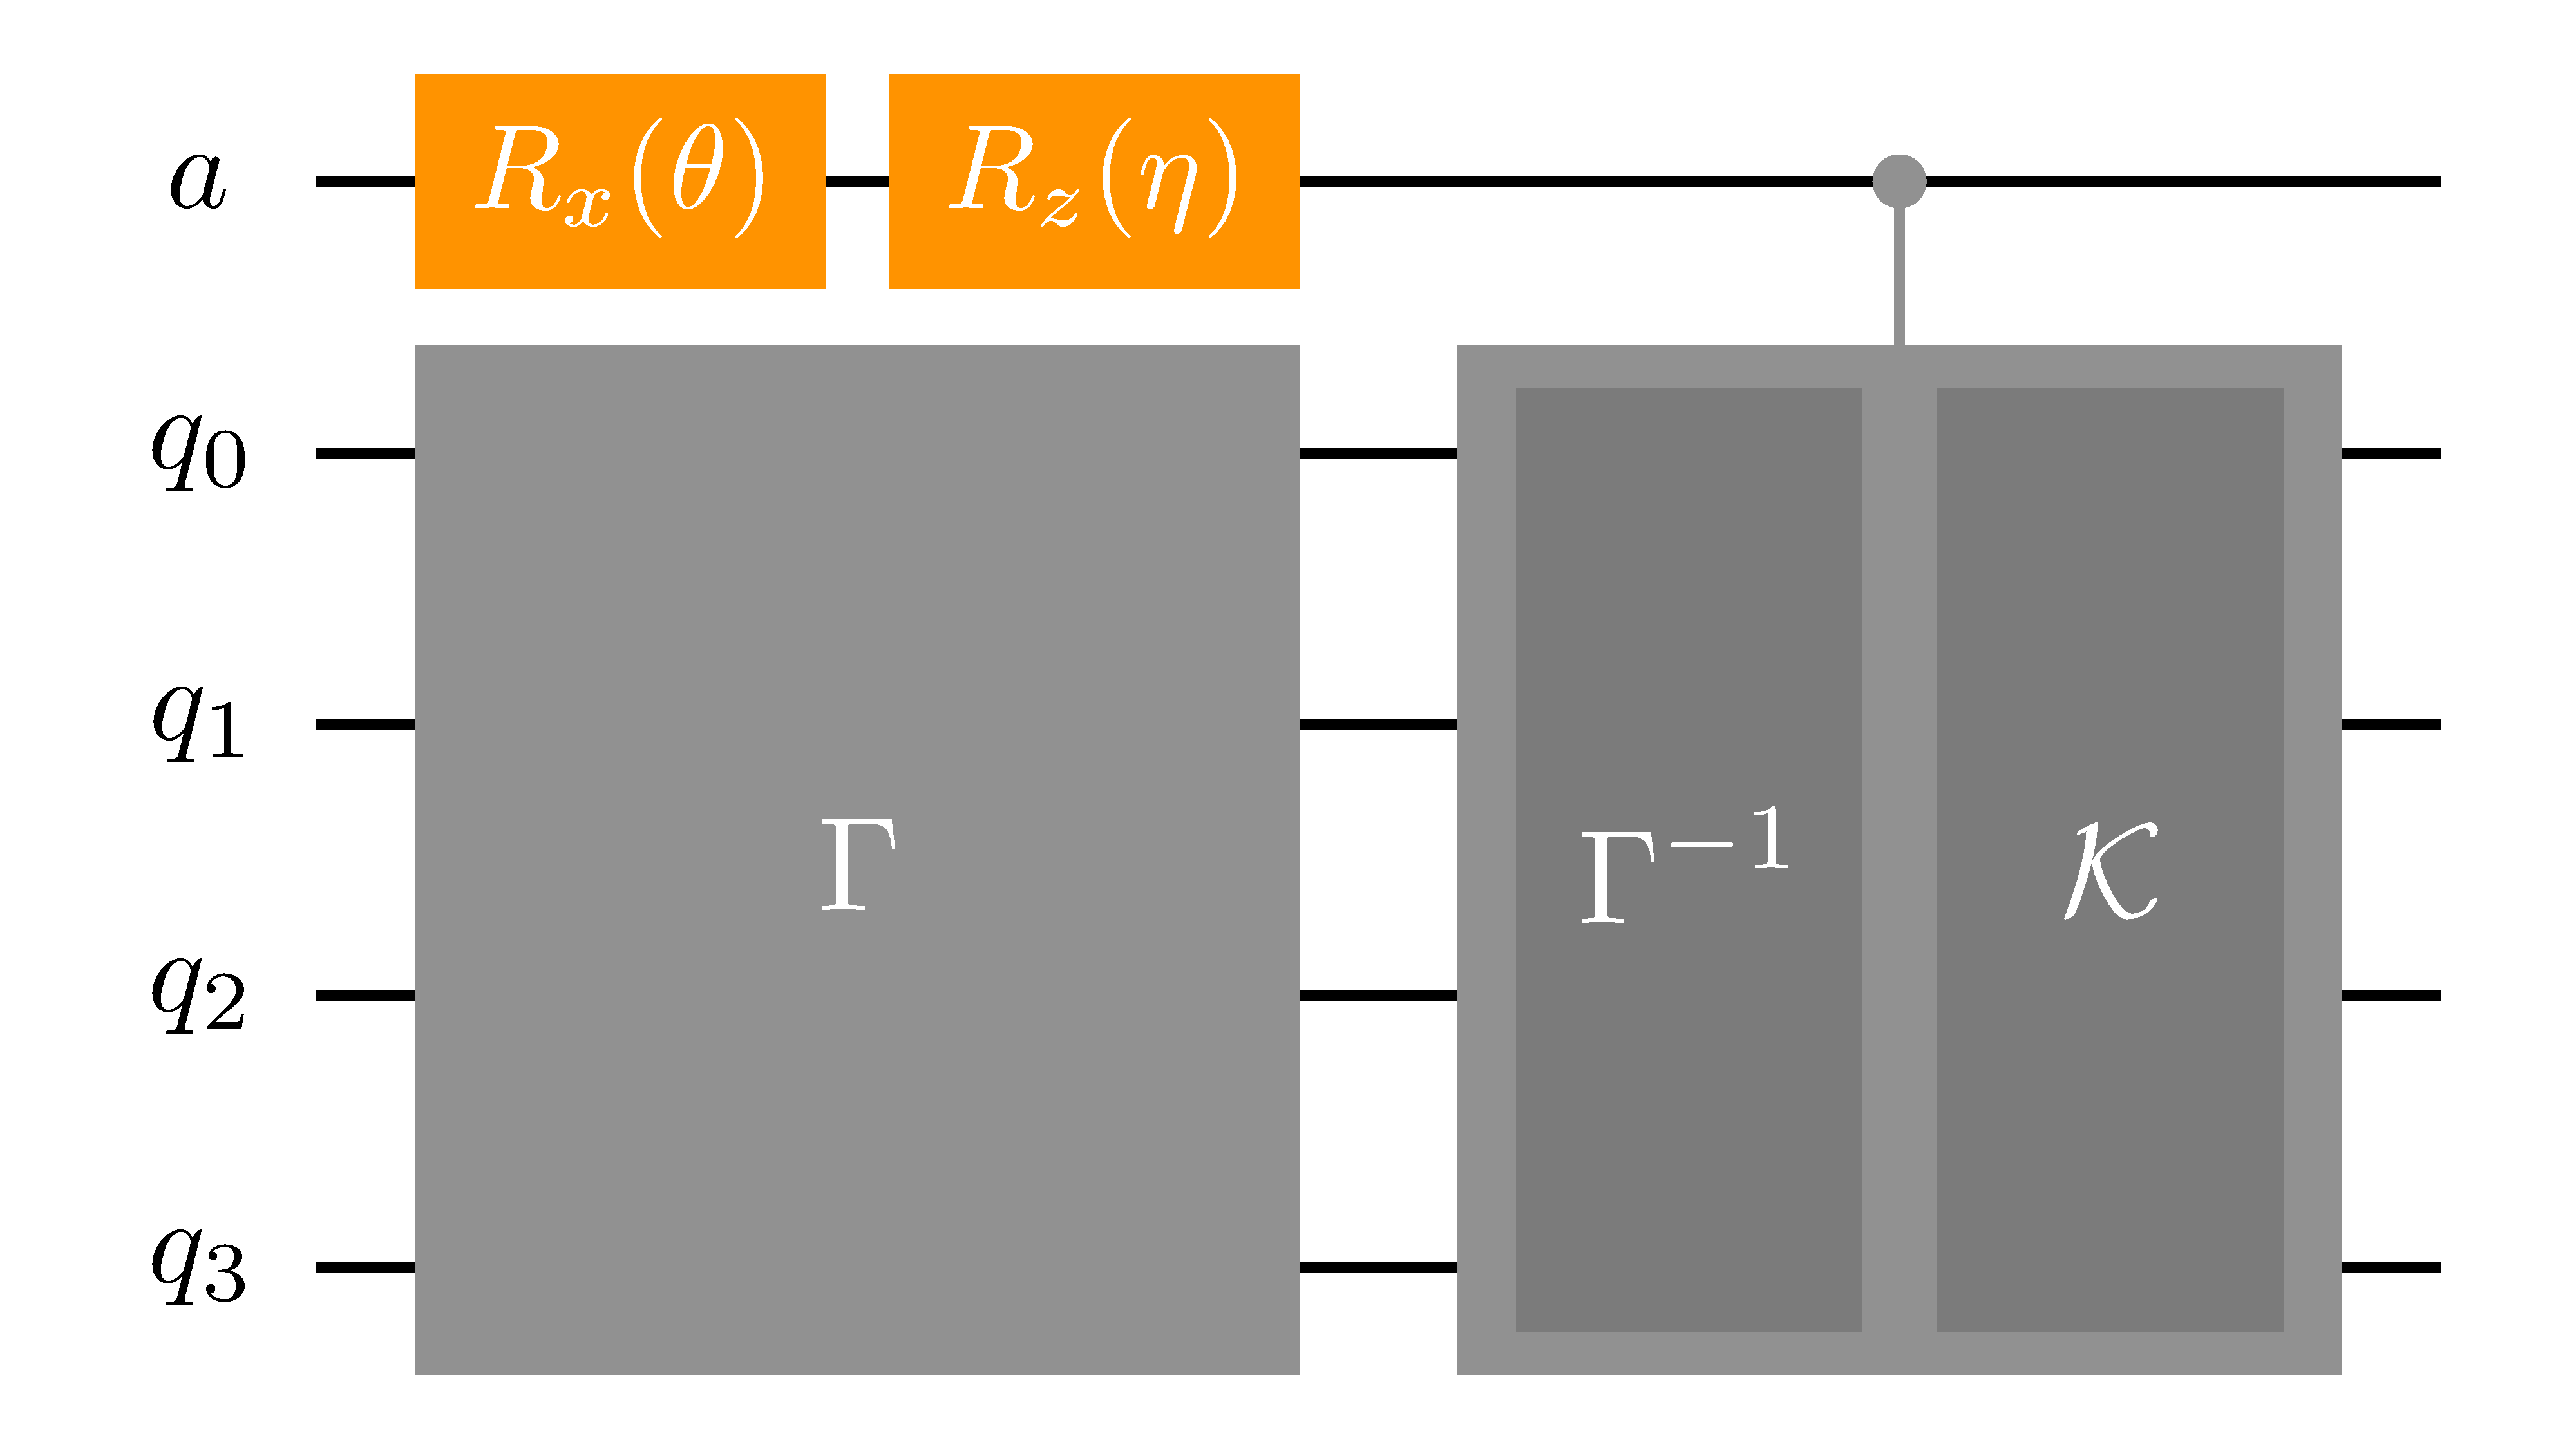
\includegraphics[width=\linewidth]{Figures/NJL1-model-solving/ansatz-implementation-ancilla-mapping}
		\end{minipage}
		\hspace{.025\linewidth}
		\begin{minipage}[c]{.45\linewidth}
			\centering
			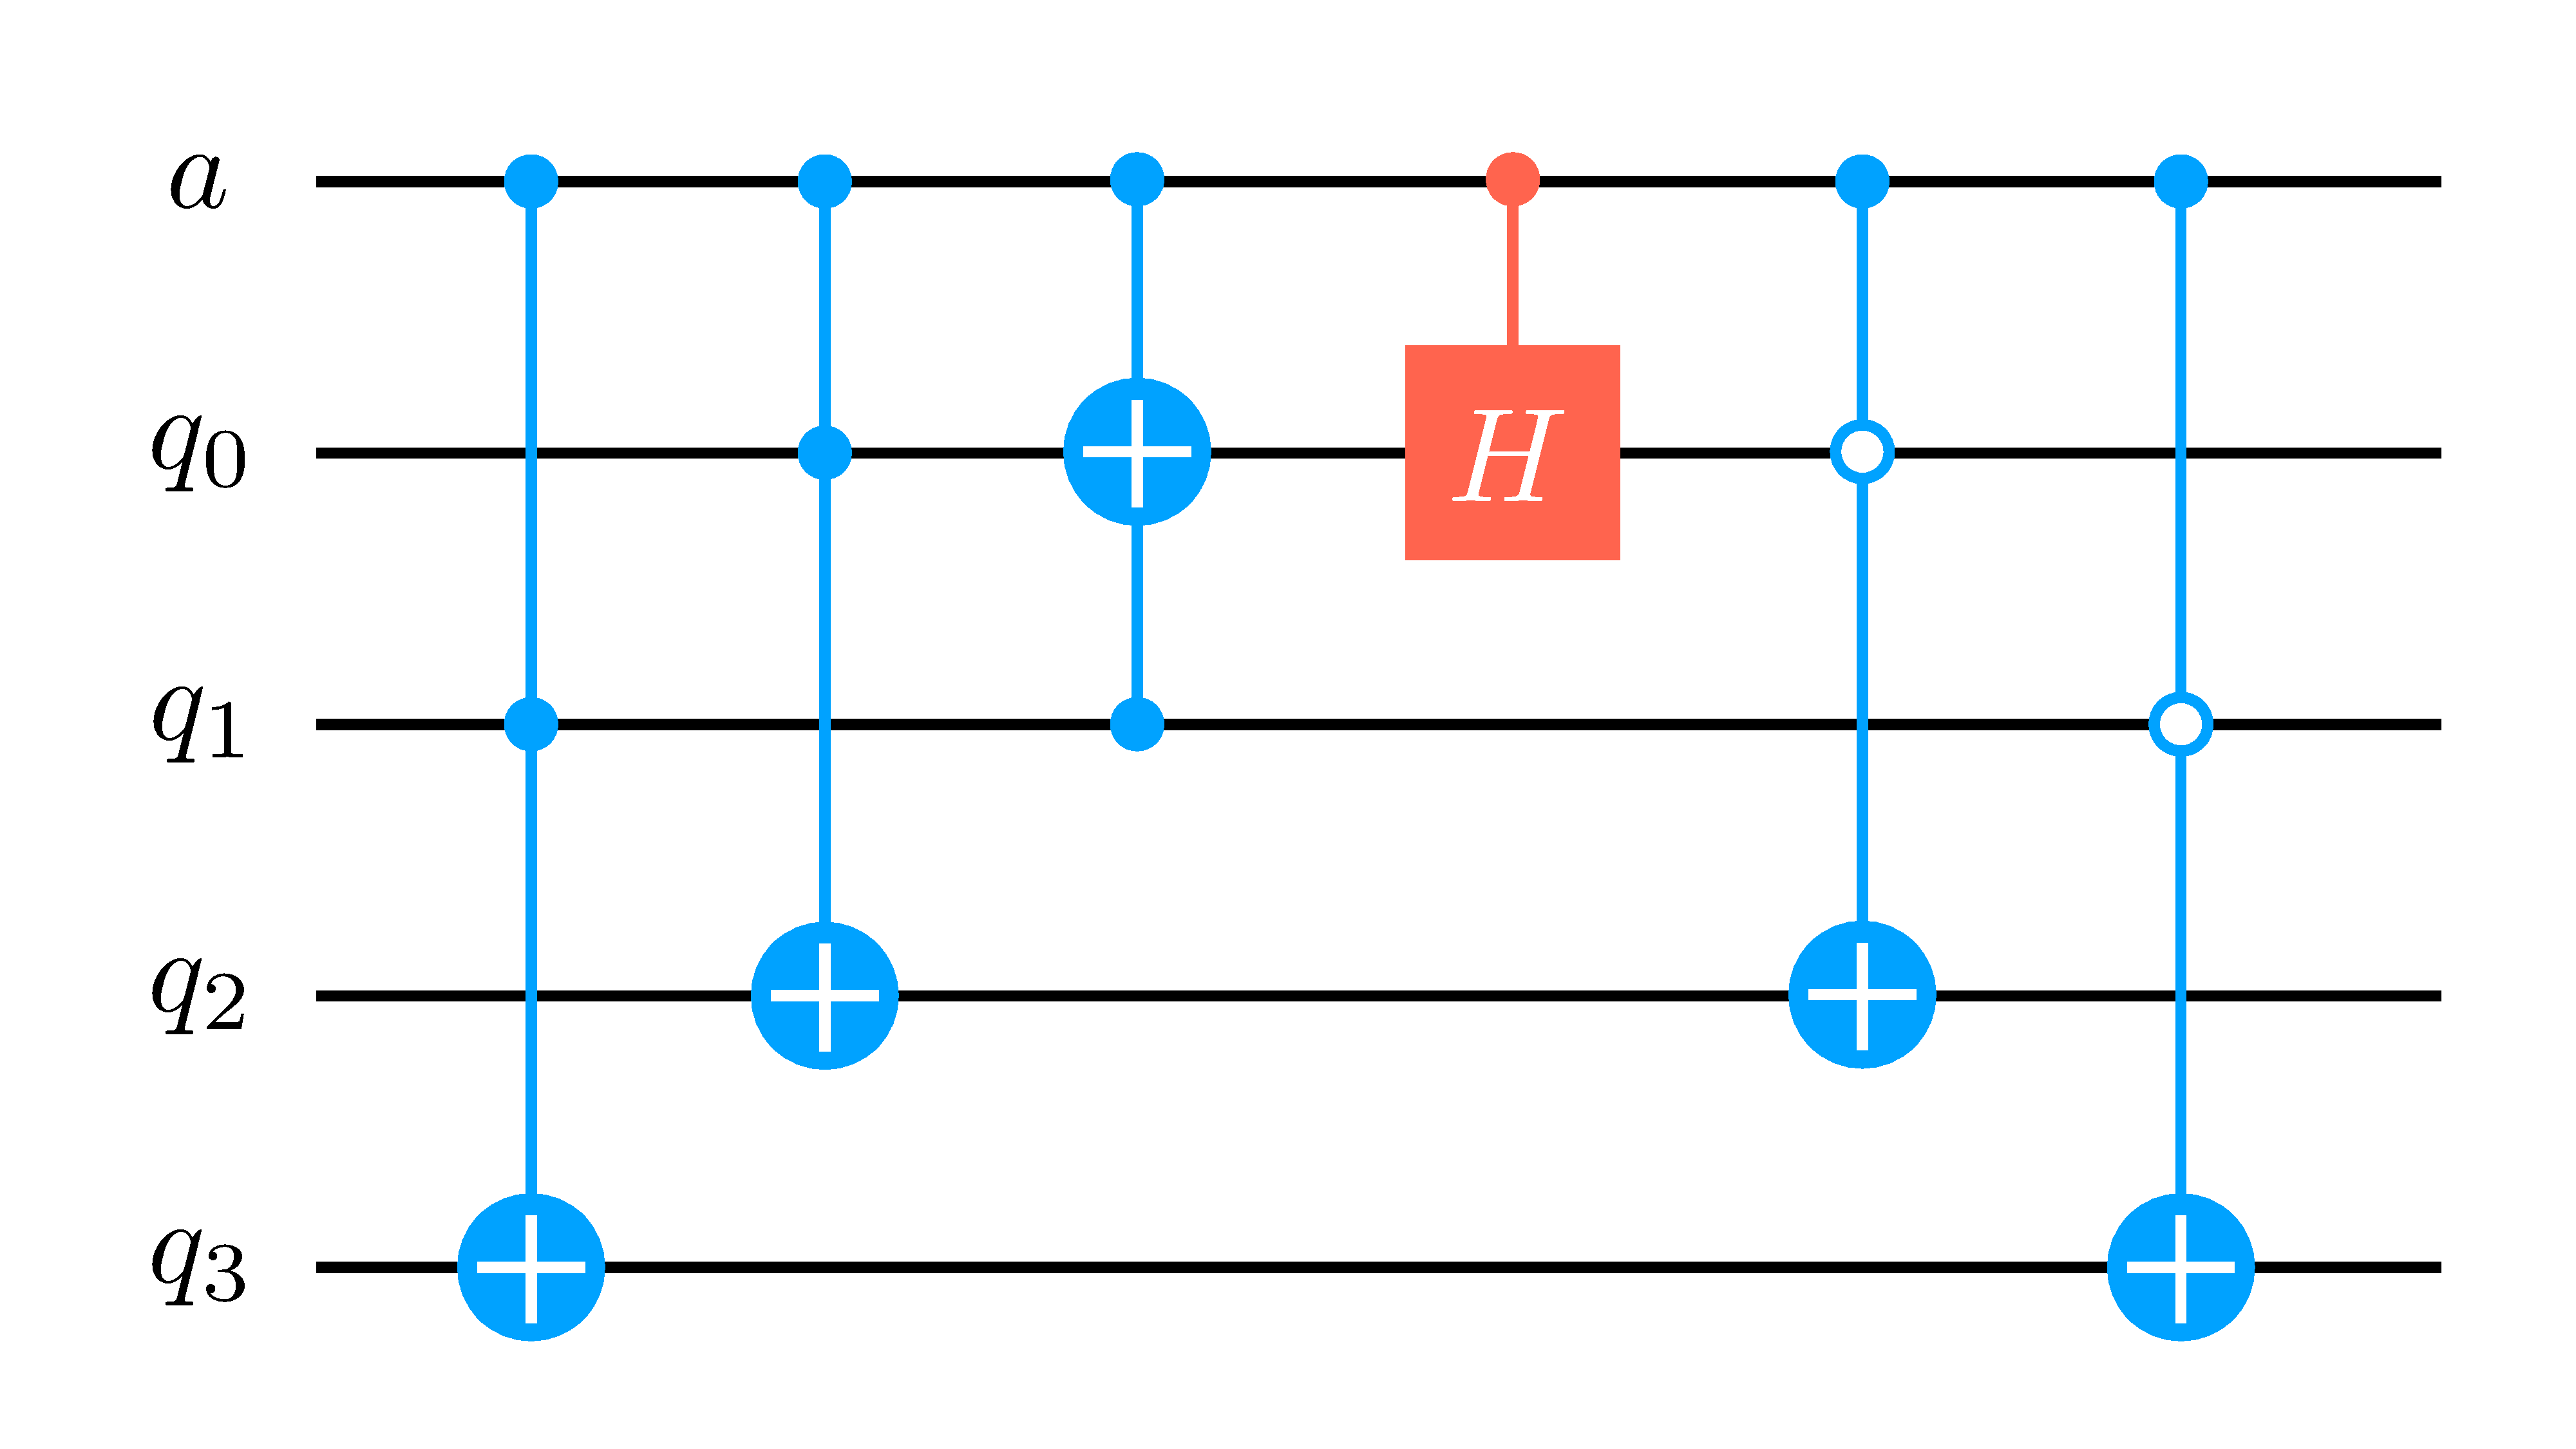
\includegraphics[width=\linewidth]{Figures/NJL1-model-solving/ansatz-implementation-controlled-gammakappa}
		\end{minipage}
		\caption{(Left) Quantum circuit to map the ancilla qubit onto the target qubit Hilbert space in our system. (Right) Simplified controlled $\mathcal{K}\Gamma^{-1}$ gate.}
	\end{figure}

%% ----------------------------------------------------------------------------
\break
%% ----------------------------------------------------------------------------

	\begin{figure}[!p]
		\centering
		\begin{minipage}[c]{.45\linewidth}
			\centering
			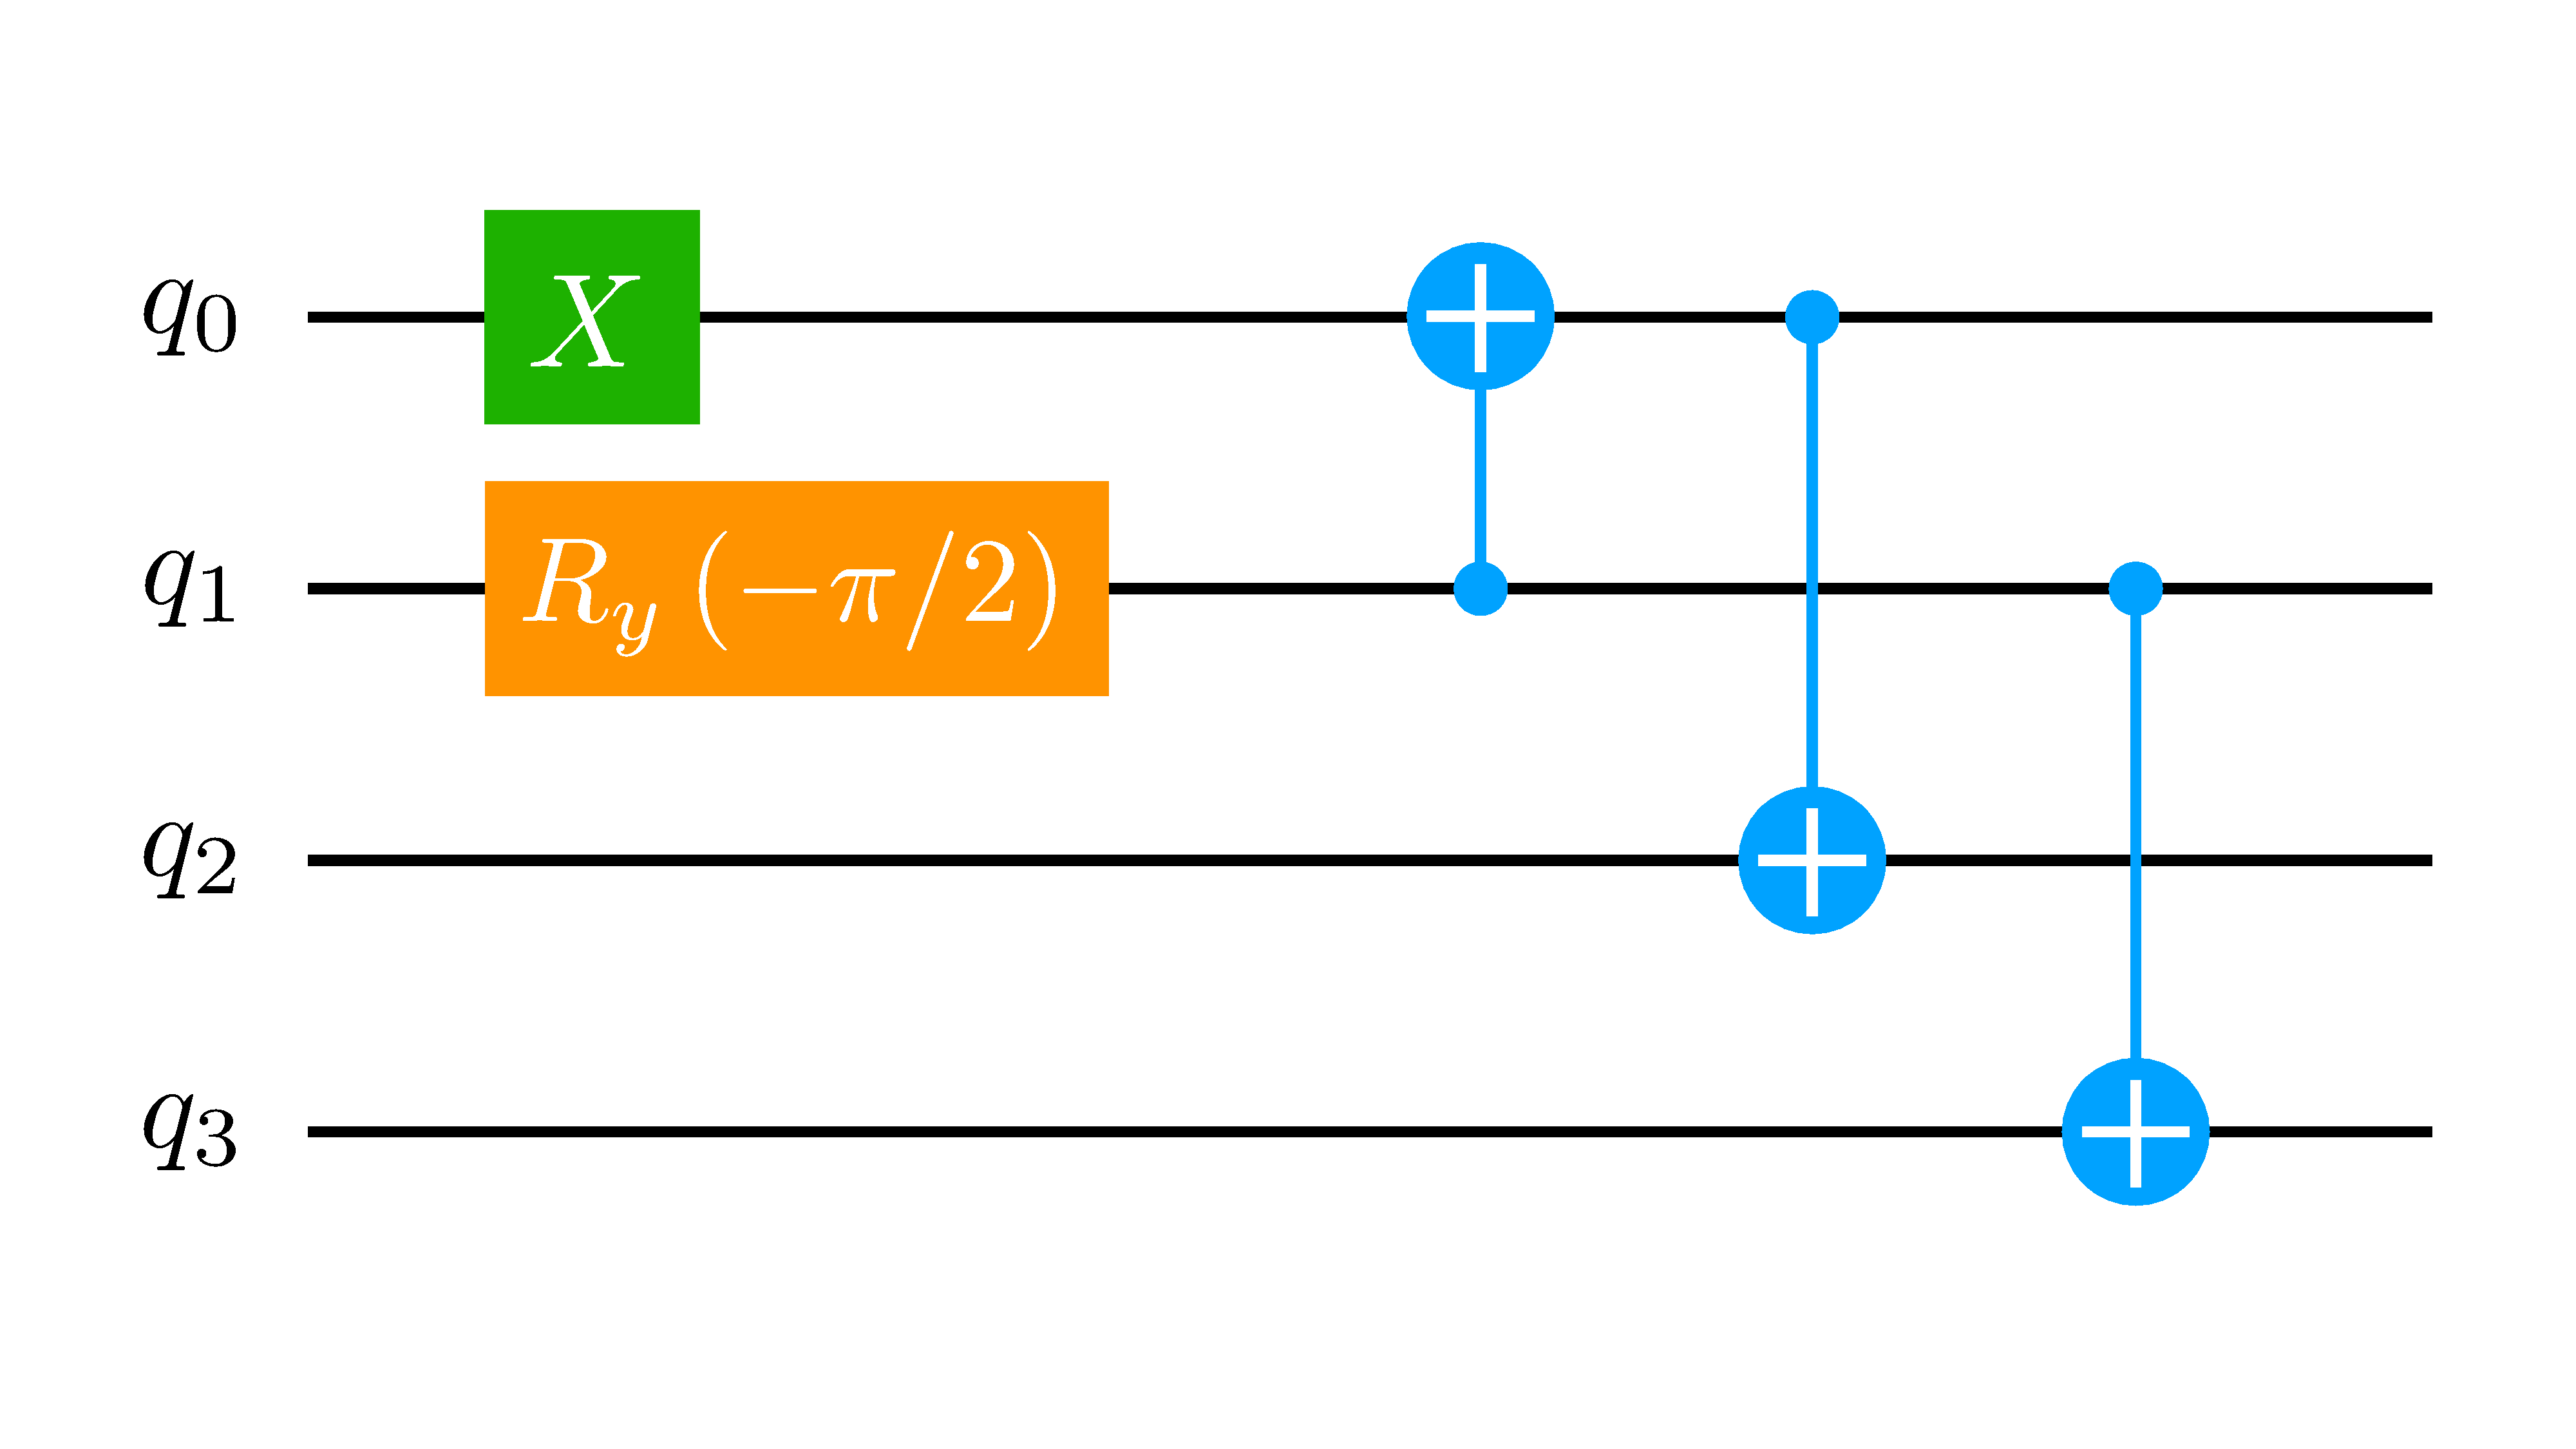
\includegraphics[width=\linewidth]{Figures/NJL1-model-solving/ansatz-implementation-base-state-preparation-gamma}
		\end{minipage}
	  \hspace{.025\linewidth}
		\begin{minipage}[c]{.45\linewidth}
			\centering
			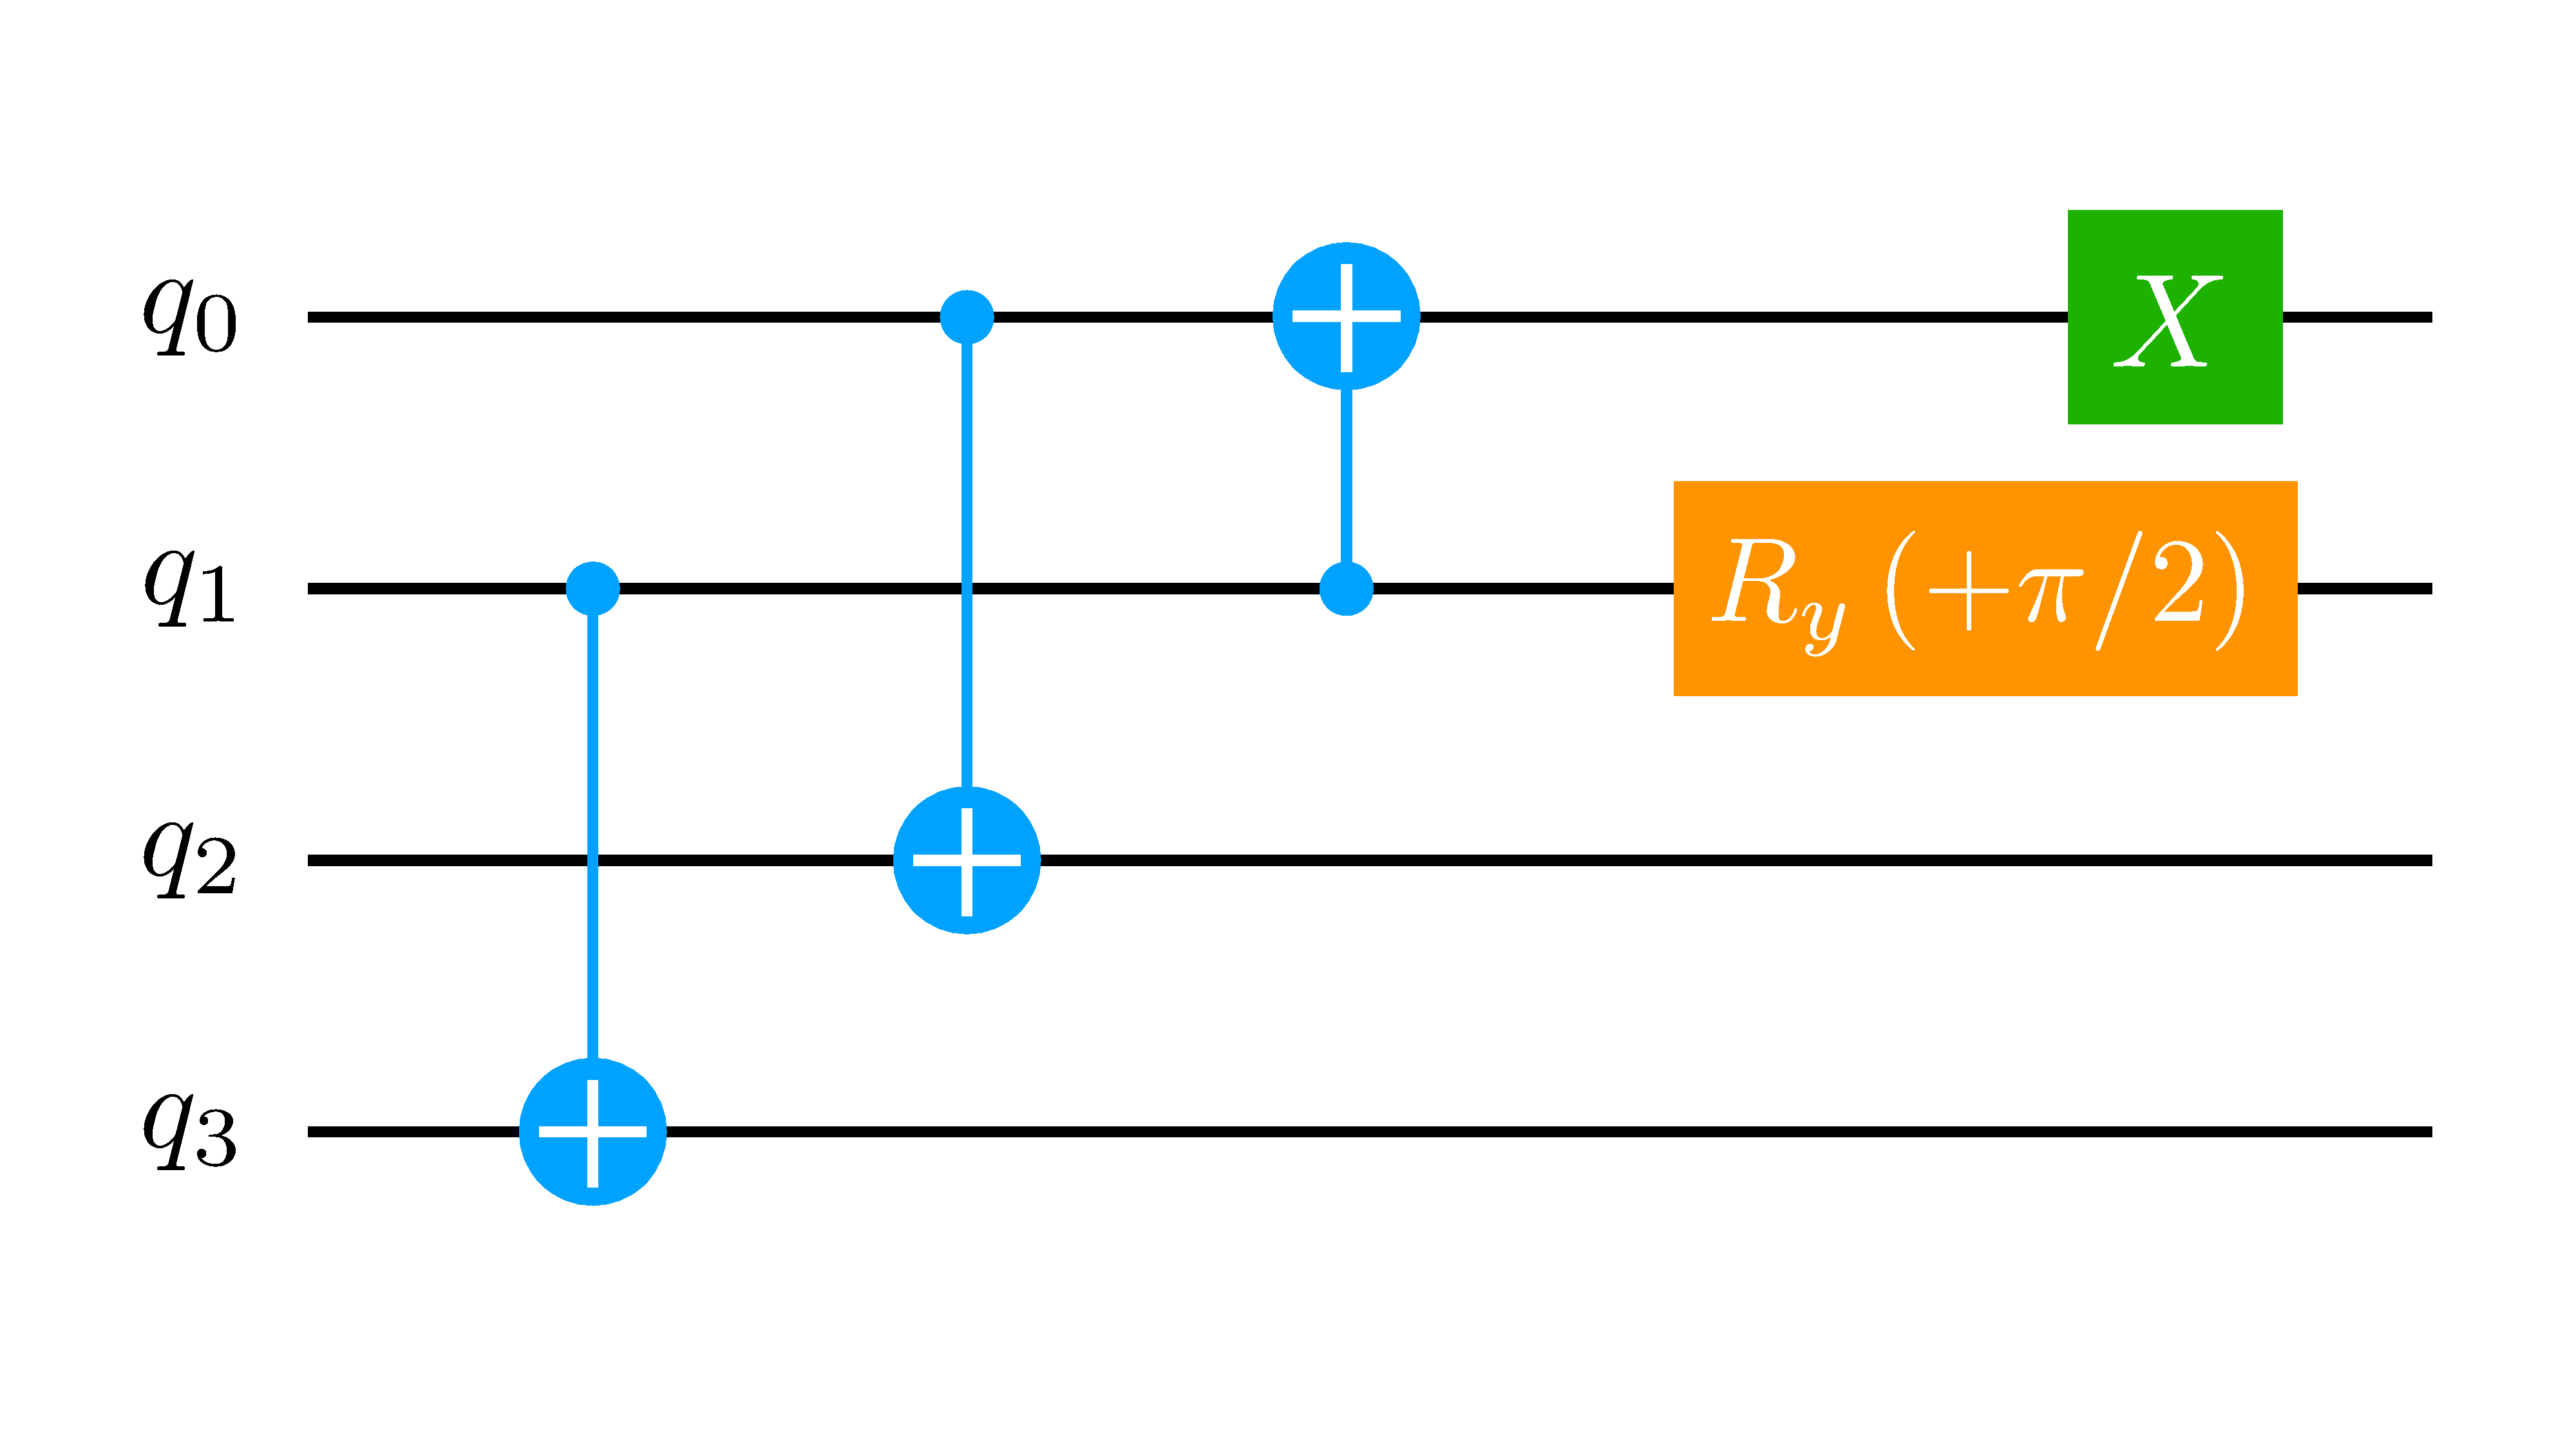
\includegraphics[width=\linewidth]{Figures/NJL1-model-solving/ansatz-implementation-base-state-reversing-gamma}
		\end{minipage}
		\caption{(Left) Preparation $\Gamma$ of state $\ket{\gamma}$. (Right) Quantum gate $\Gamma^{-1}$ for reversing state $\ket{\gamma}$.}
	\end{figure}

%% ----------------------------------------------------------------------------
\break
%% ----------------------------------------------------------------------------

	\begin{figure}[!p]
		\centering
		\begin{minipage}[c]{.45\linewidth}
			\centering
			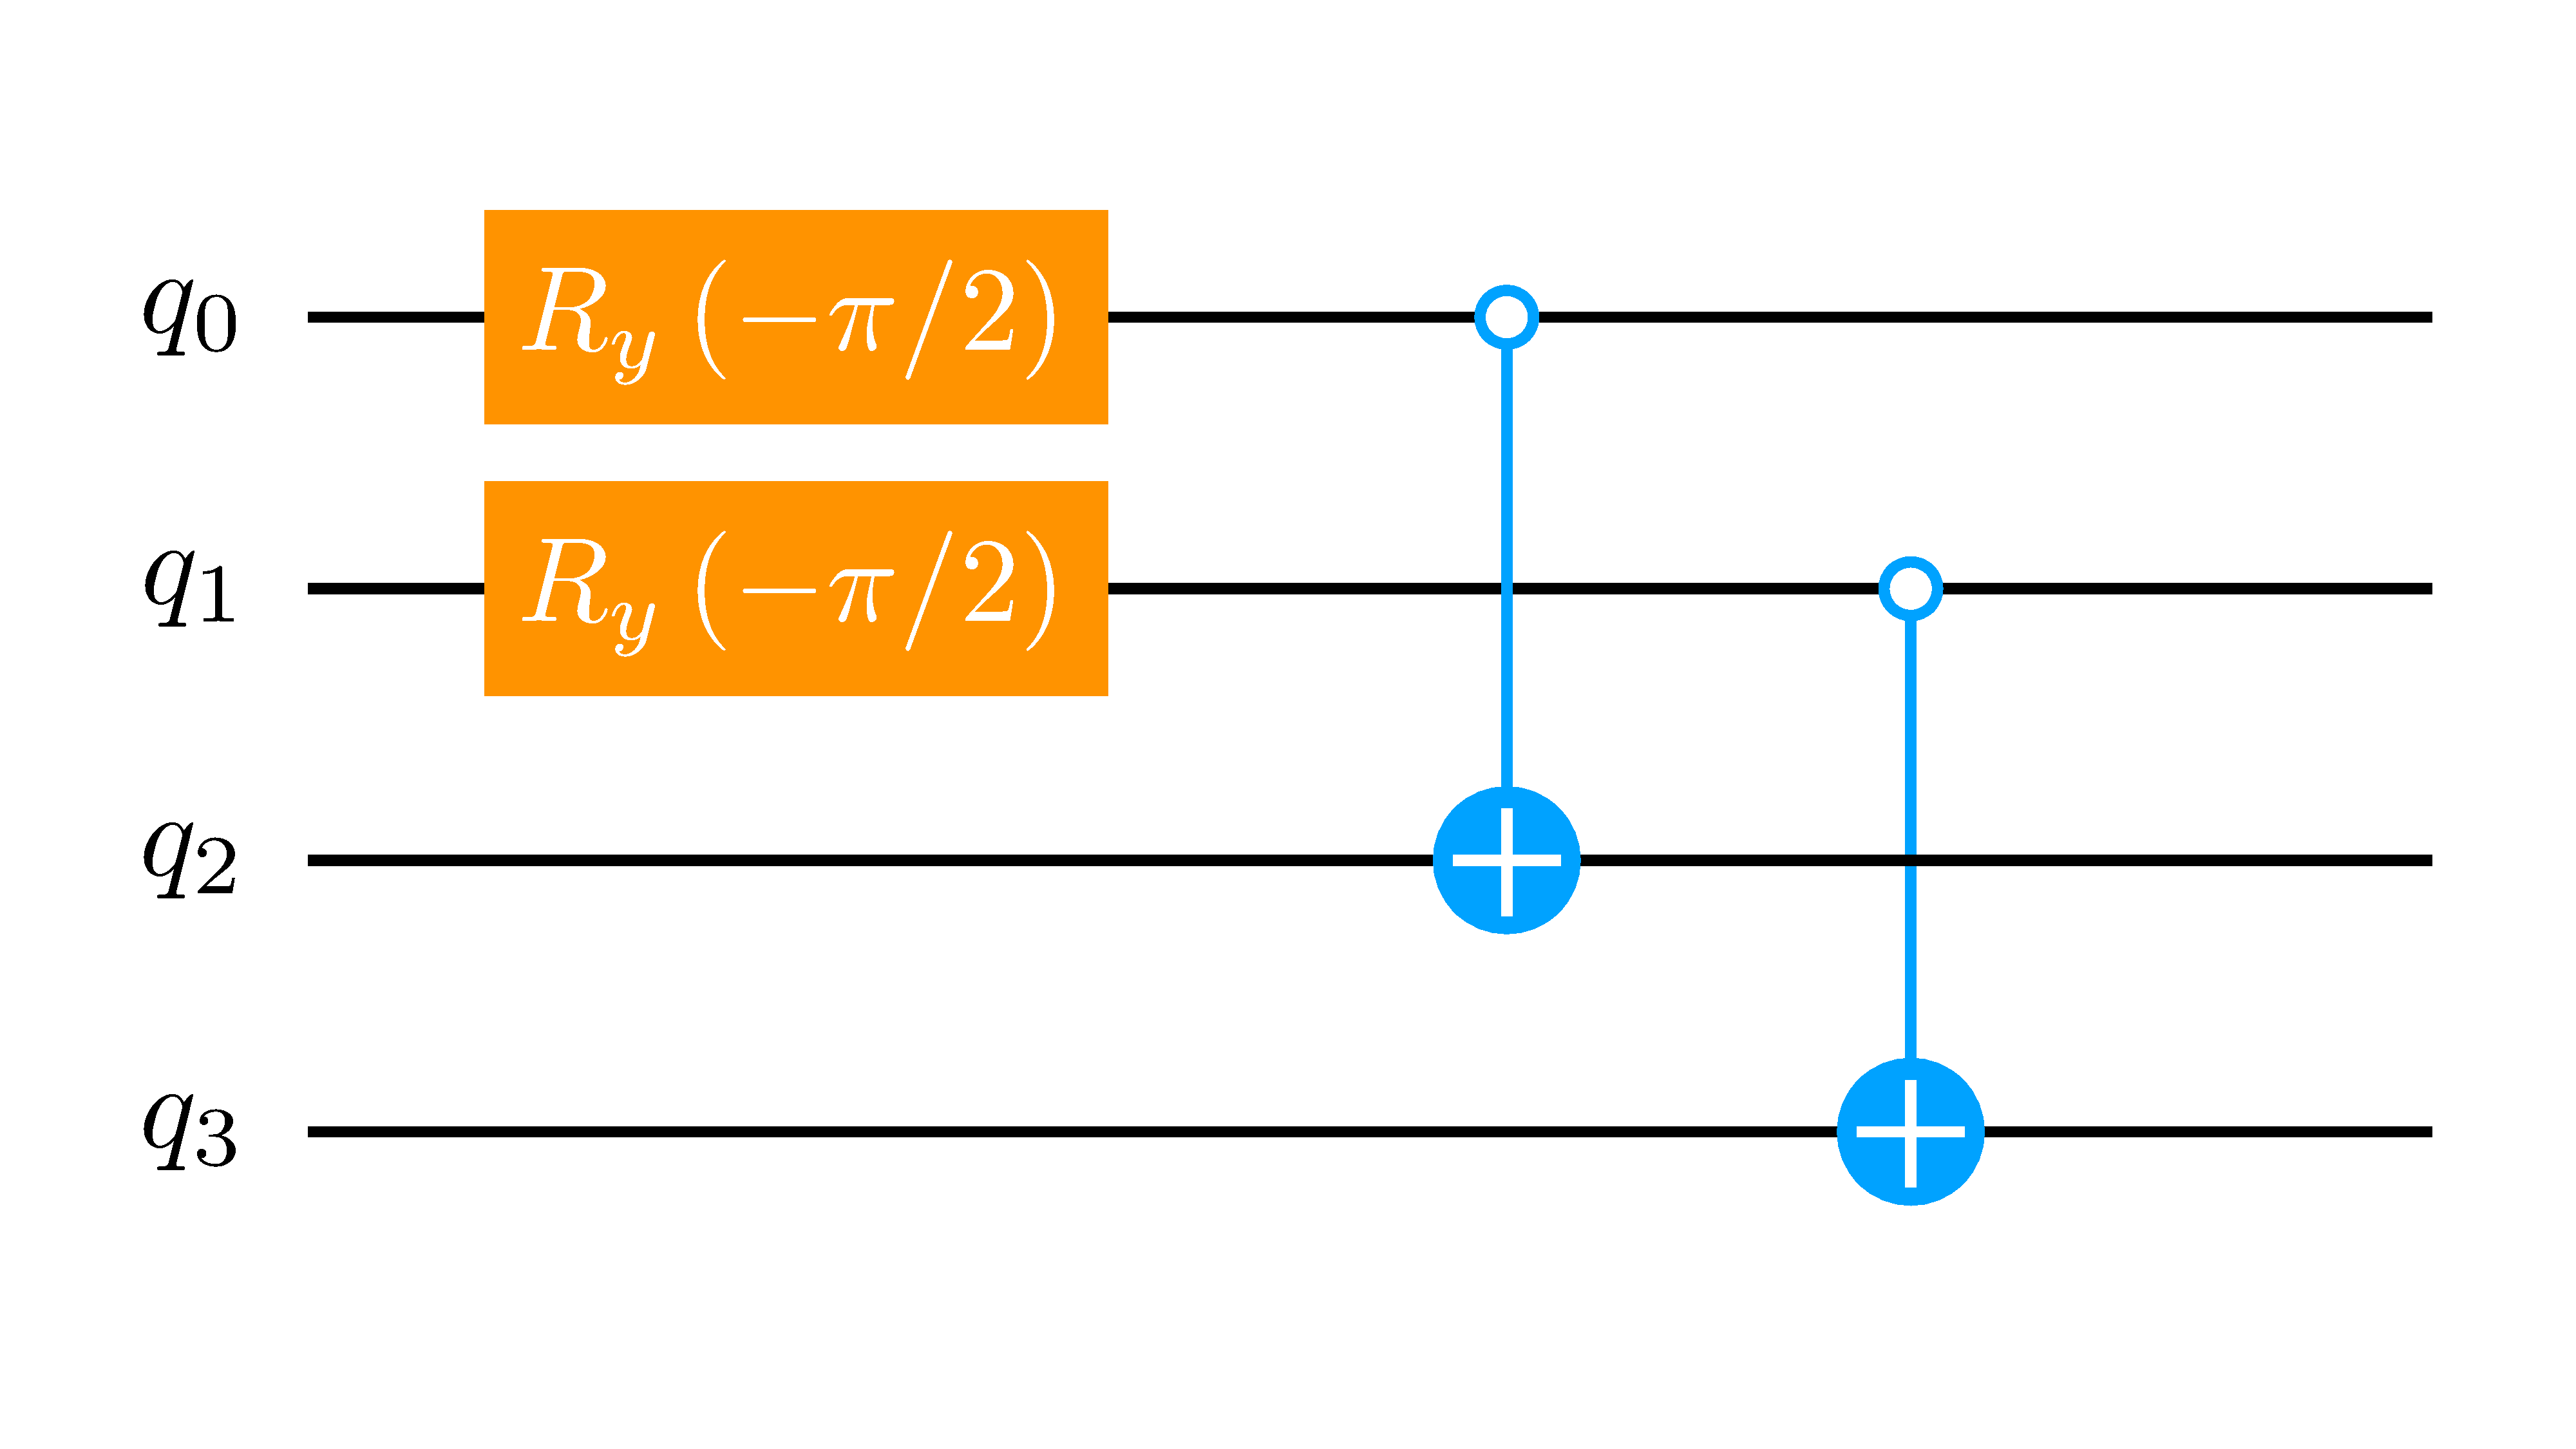
\includegraphics[width=\linewidth]{Figures/NJL1-model-solving/ansatz-implementation-base-state-preparation-kappa}
		\end{minipage}
	  \hspace{.025\linewidth}
		\begin{minipage}[c]{.45\linewidth}
			\centering
			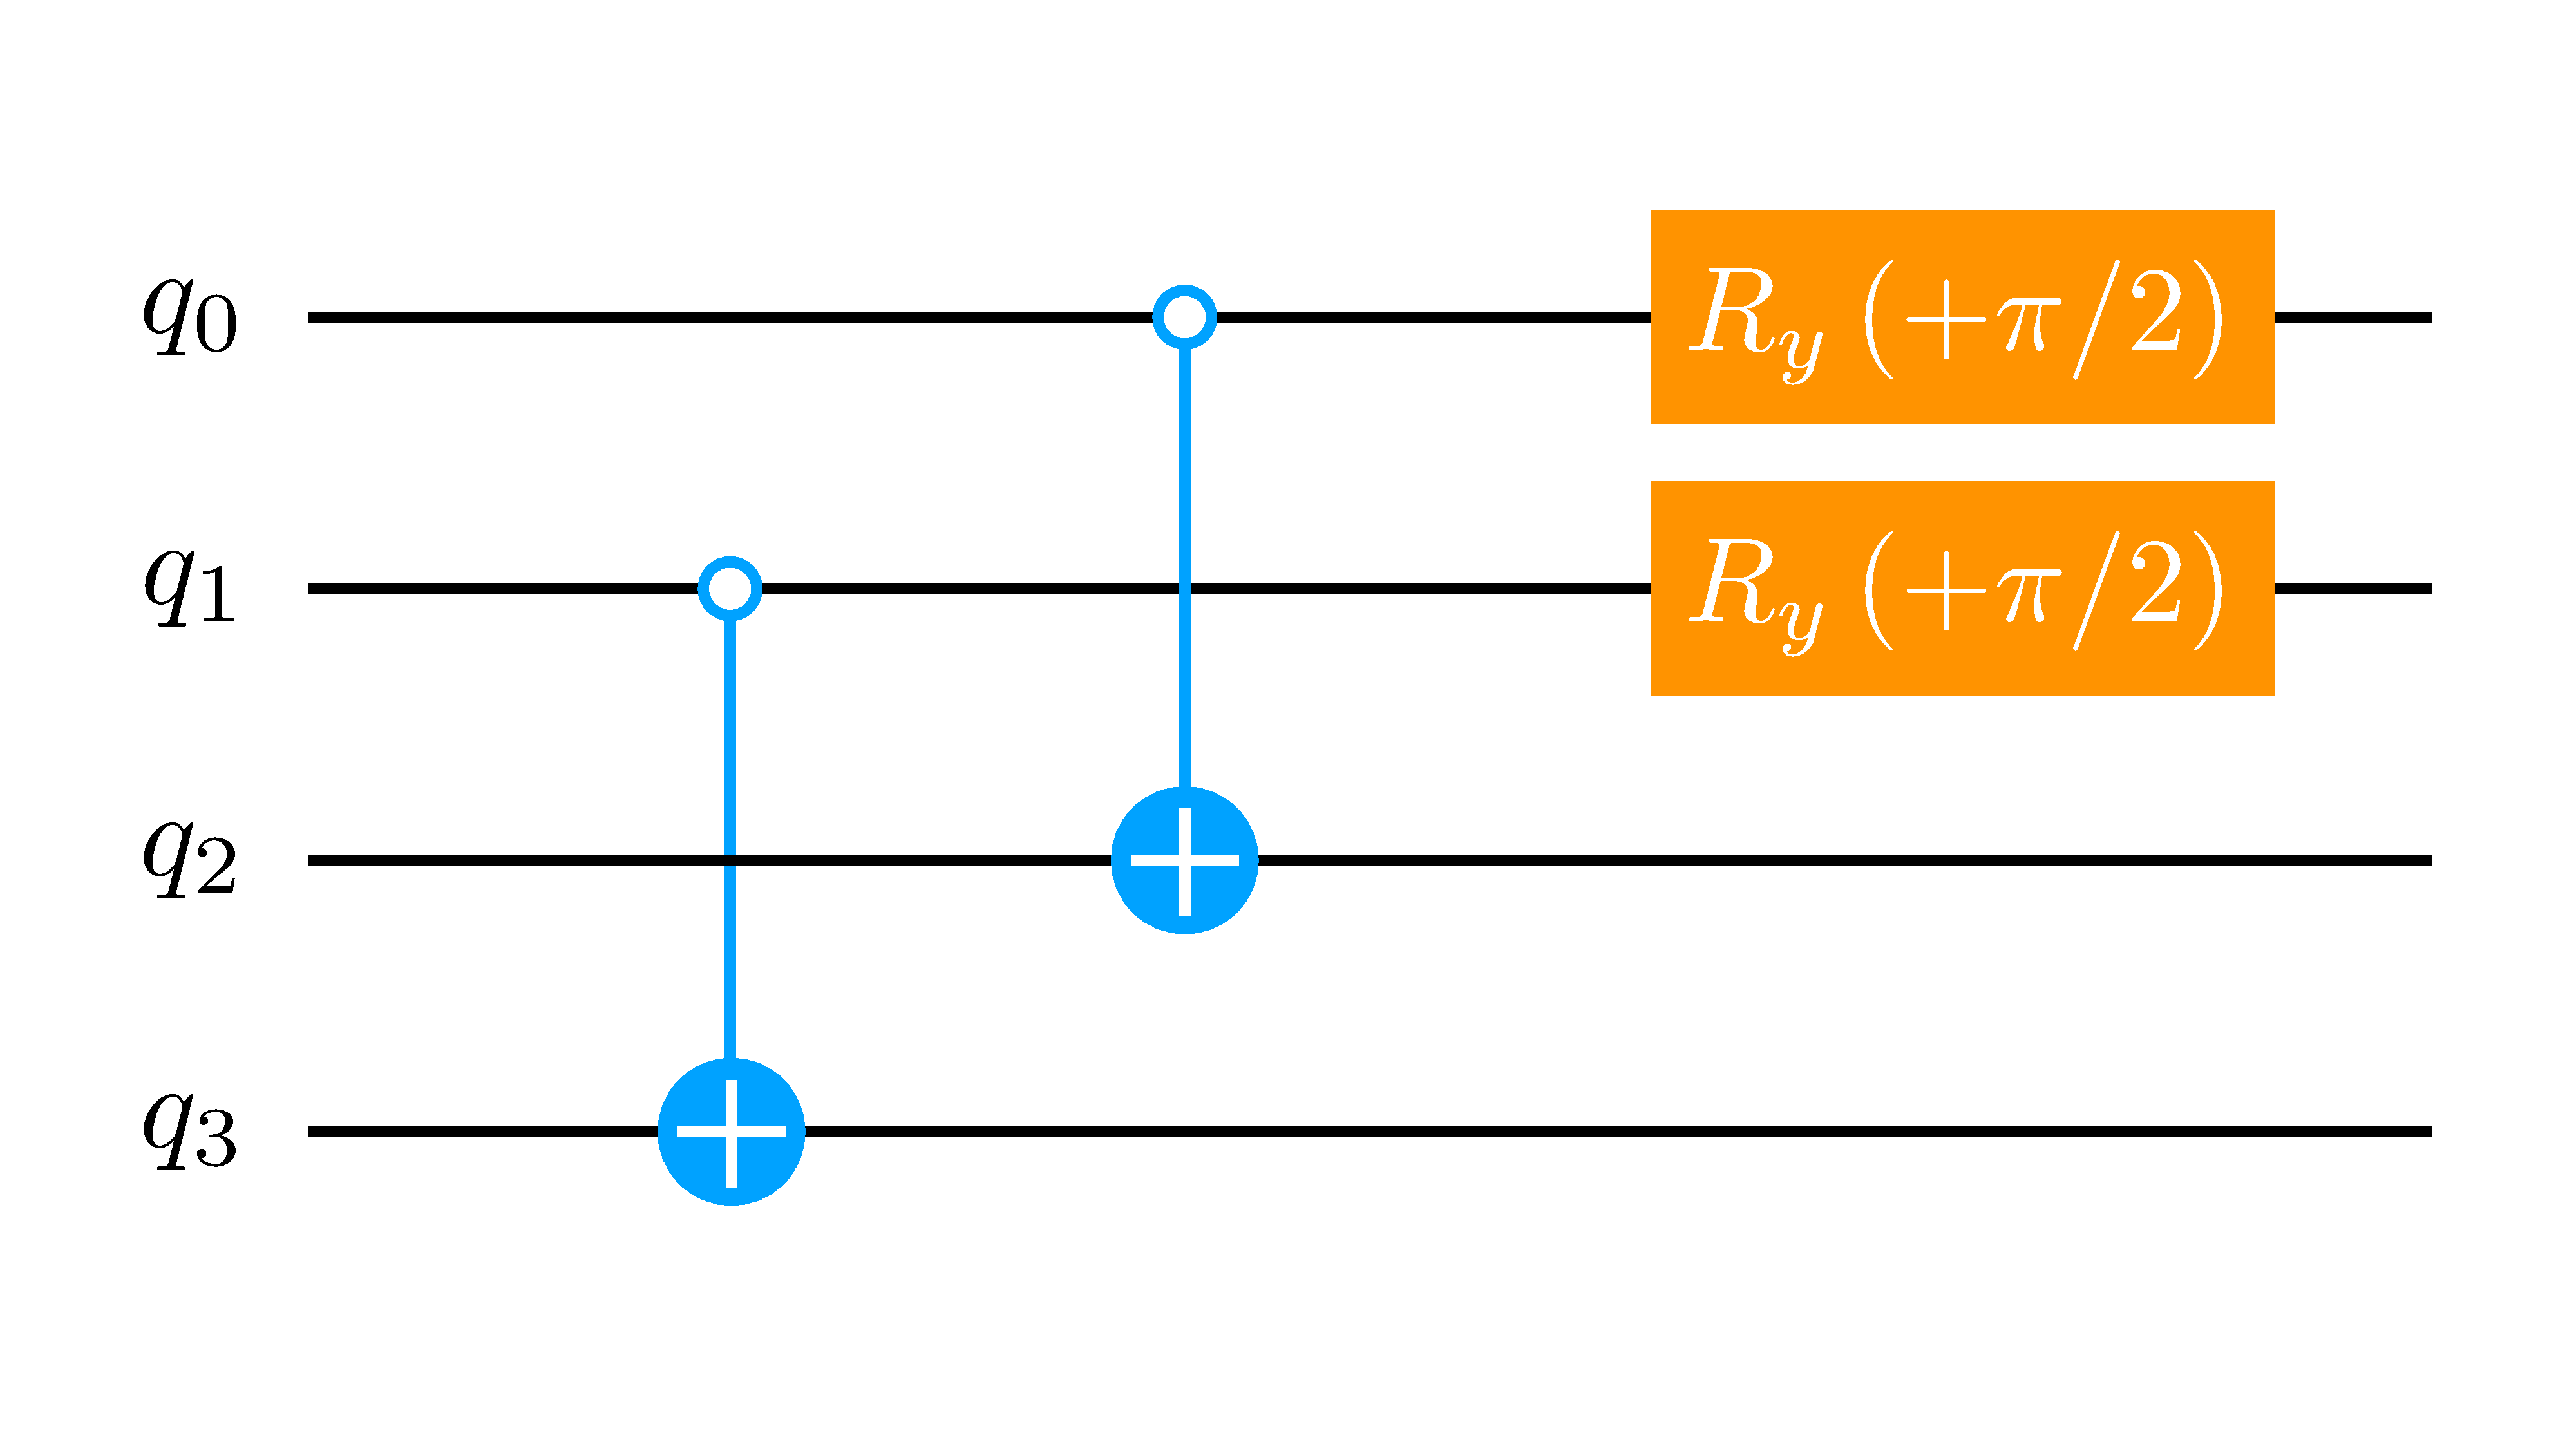
\includegraphics[width=\linewidth]{Figures/NJL1-model-solving/ansatz-implementation-base-state-reversing-kappa}
		\end{minipage}
		\caption{(Left) Preparation $\mathcal{K}$ of state $\ket{\kappa}$. (Right) Quantum gate $\mathcal{K}^{-1}$ for reversing state $\ket{\kappa}$.}
	\end{figure}

%% ----------------------------------------------------------------------------
\break
%% ----------------------------------------------------------------------------

	\begin{multicols}{2}

		This parametrization will work if we are interested in measuring in the computational basis only (i.e. Pauli-Z measurements). Nonetheless, if we change our basis before measuring (e.g. to Pauli-X or Pauli-Y) we are going to face a problem: the resulting states of our system will be entangled with the ancilla qubit, and so, states that should be indistinguishable from one another will turn out distinct; because of this, the probability distributions will not be correct.

		\begin{gather*}
		  \text{Pr} \qty(\ket{\psi}_{\text{distinct}}) =
		    \norm{\psi_\gamma}^2 + \norm{\psi_\kappa}^2 \\
		  \text{Pr} \qty(\ket{\psi}_{\text{indist}}) =
		    \norm{\psi_\gamma + \psi_\kappa}^2 \\
		  \text{Pr} \qty(\ket{\psi}_{\text{distinct}}) \geq
		    \text{Pr} \qty(\ket{\psi}_{\text{indist}})
		\end{gather*}

		\columnbreak

		Therefore, as a last step, we need to \textbf{break this entanglement}.

		\begin{center}
			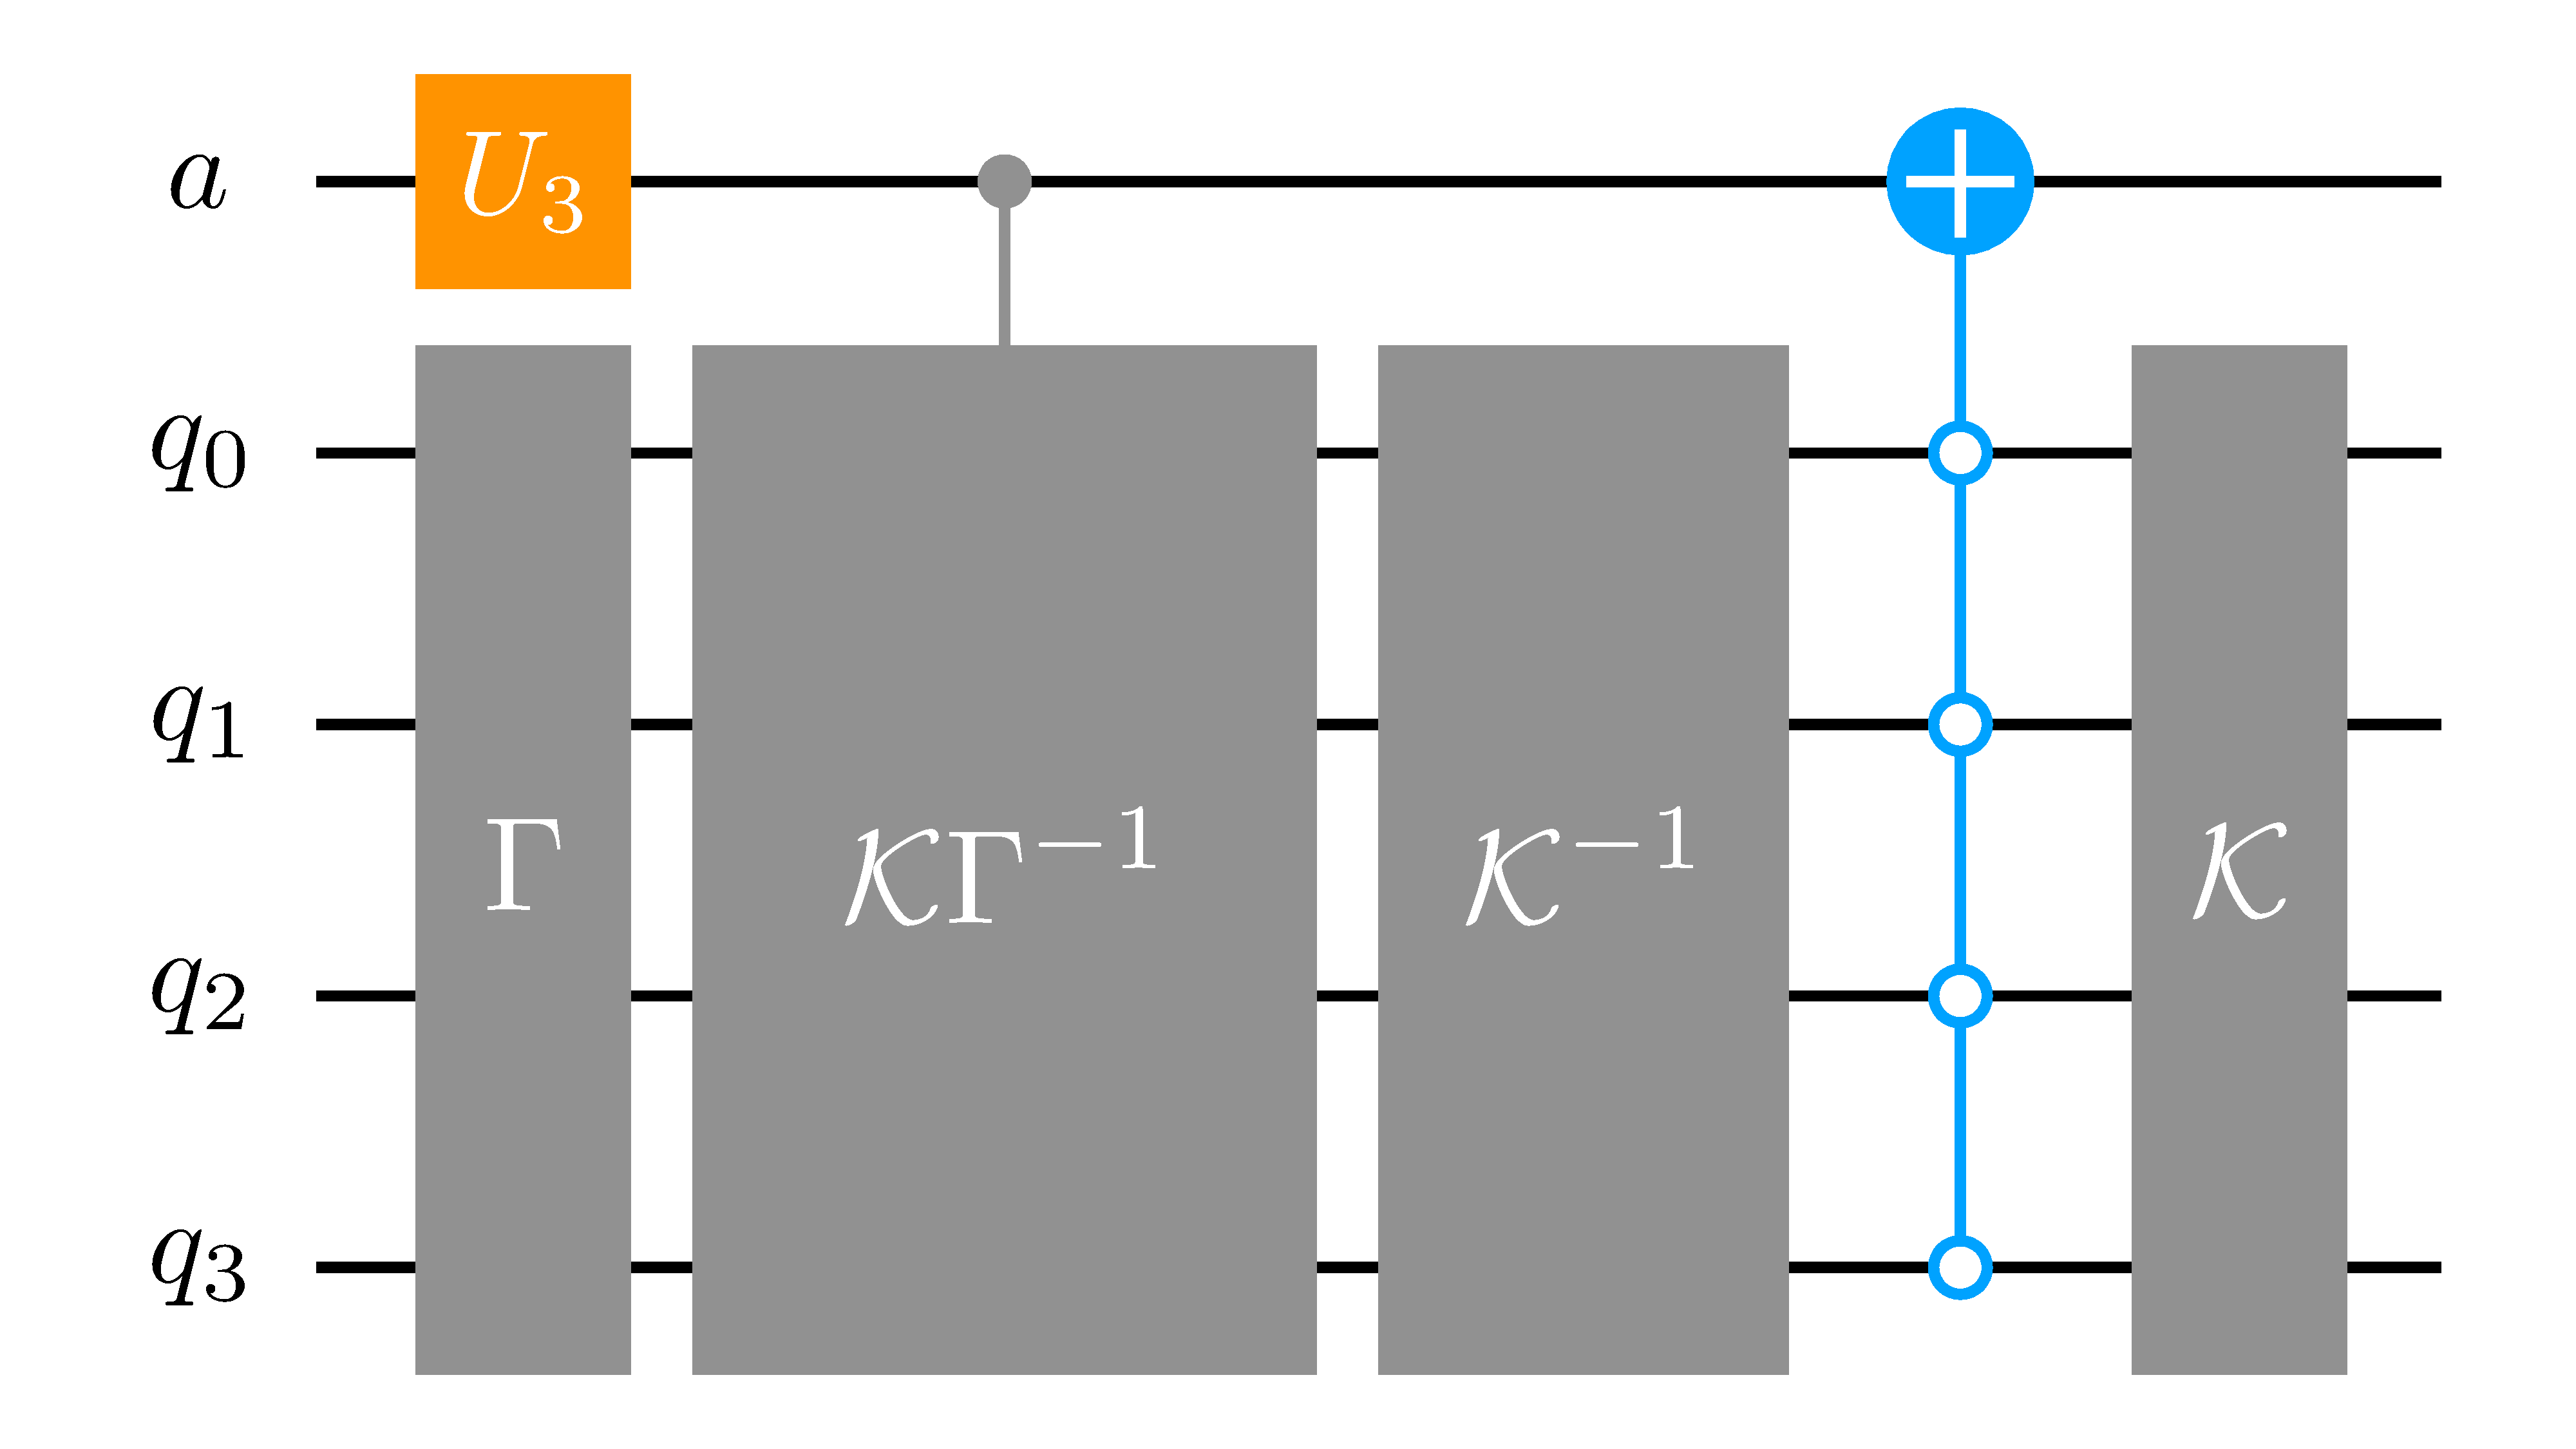
\includegraphics[width=.4\paperwidth]{Figures/NJL1-model-solving/ansatz-implementation-circuit}
		\end{center}

	\end{multicols}

\end{frame}

%% ----------------------------------------------------------------------------
%% ----------------------------------------------------------------------------

\begin{frame}[allowframebreaks]{Ground state energy}

	At long last, we have everything that we need to solve for the ground state energy of our system using a quantum computer. For simplicity, we will do so first through a \textbf{quantum simulator}.

	\begin{center}
		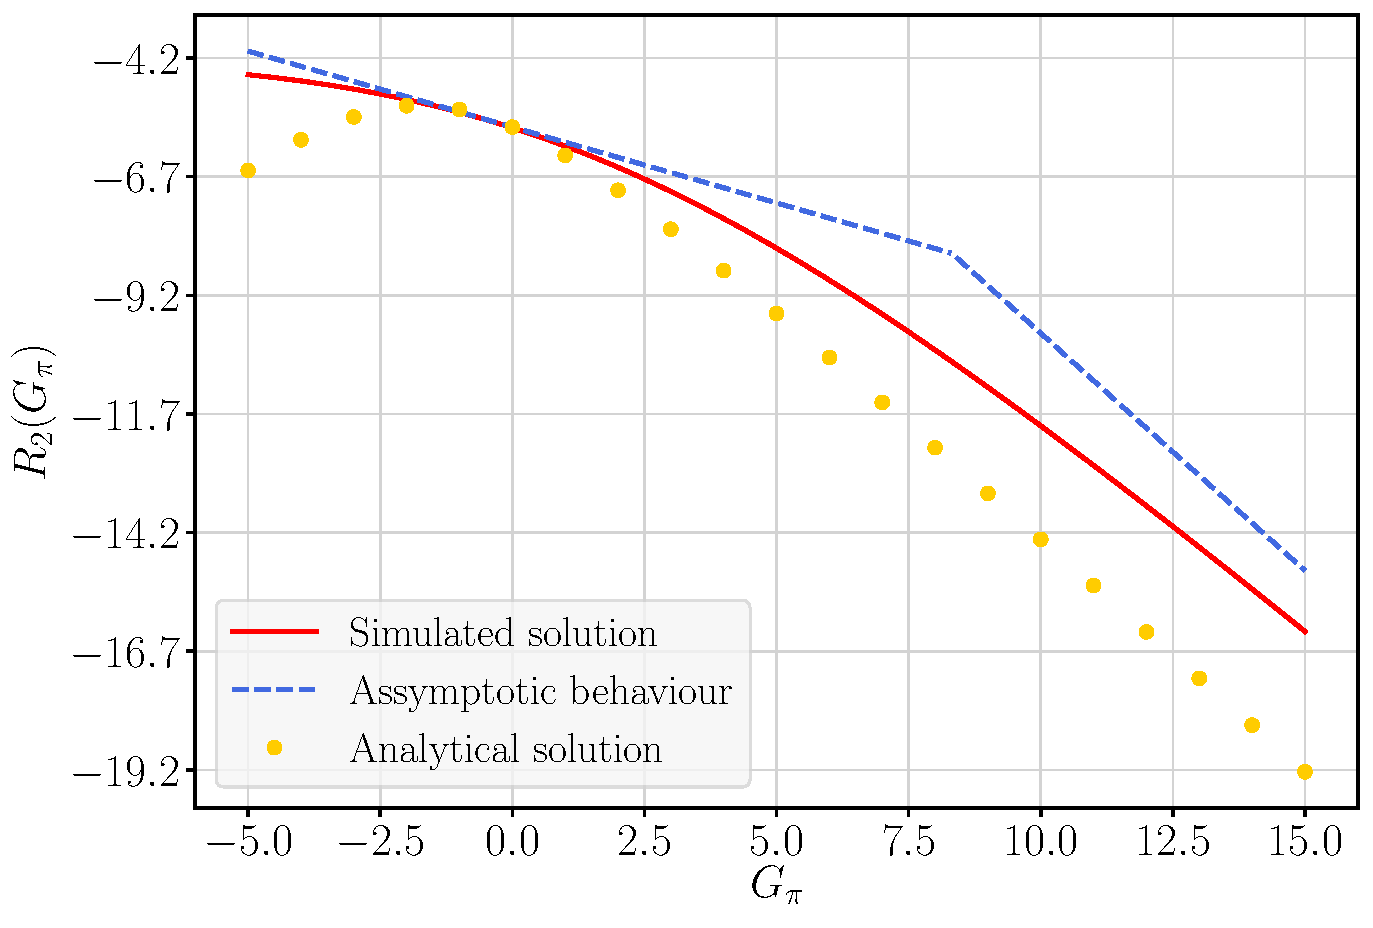
\includegraphics[width=.45\paperwidth]{Figures/chapter05/G2}
	\end{center}
	\vspace{-2em}

%% ----------------------------------------------------------------------------
\break
%% ----------------------------------------------------------------------------

	\begin{figure}[!p]
		\centering
		\begin{minipage}[c]{.4\linewidth}
			\centering
			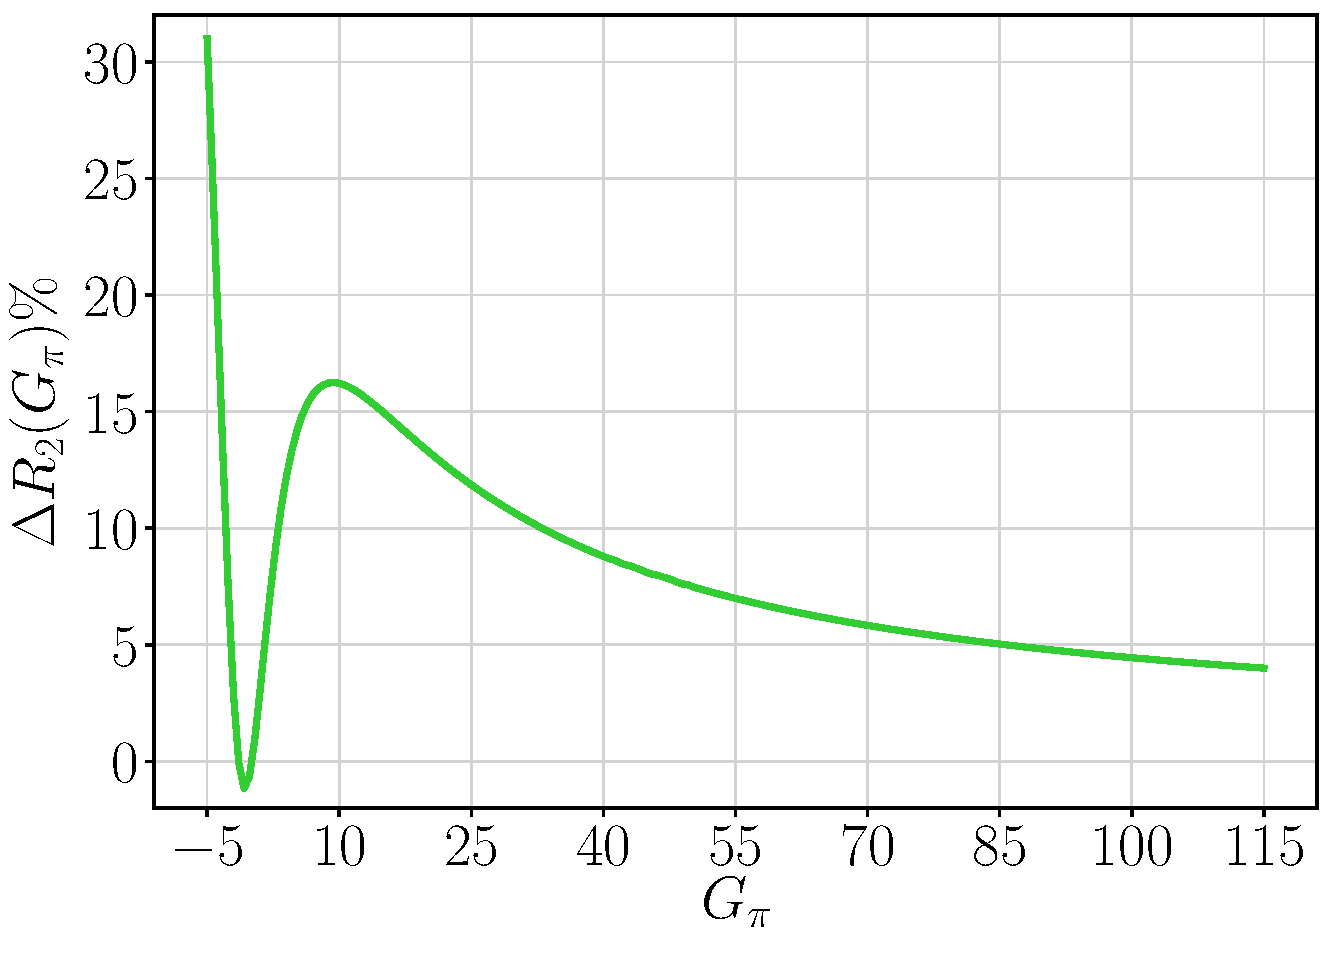
\includegraphics[width=.8\linewidth]{Figures/chapter05/G2-err}
		\end{minipage}
		\hspace{.025\linewidth}
		\begin{minipage}[c]{.4\linewidth}
			\centering
			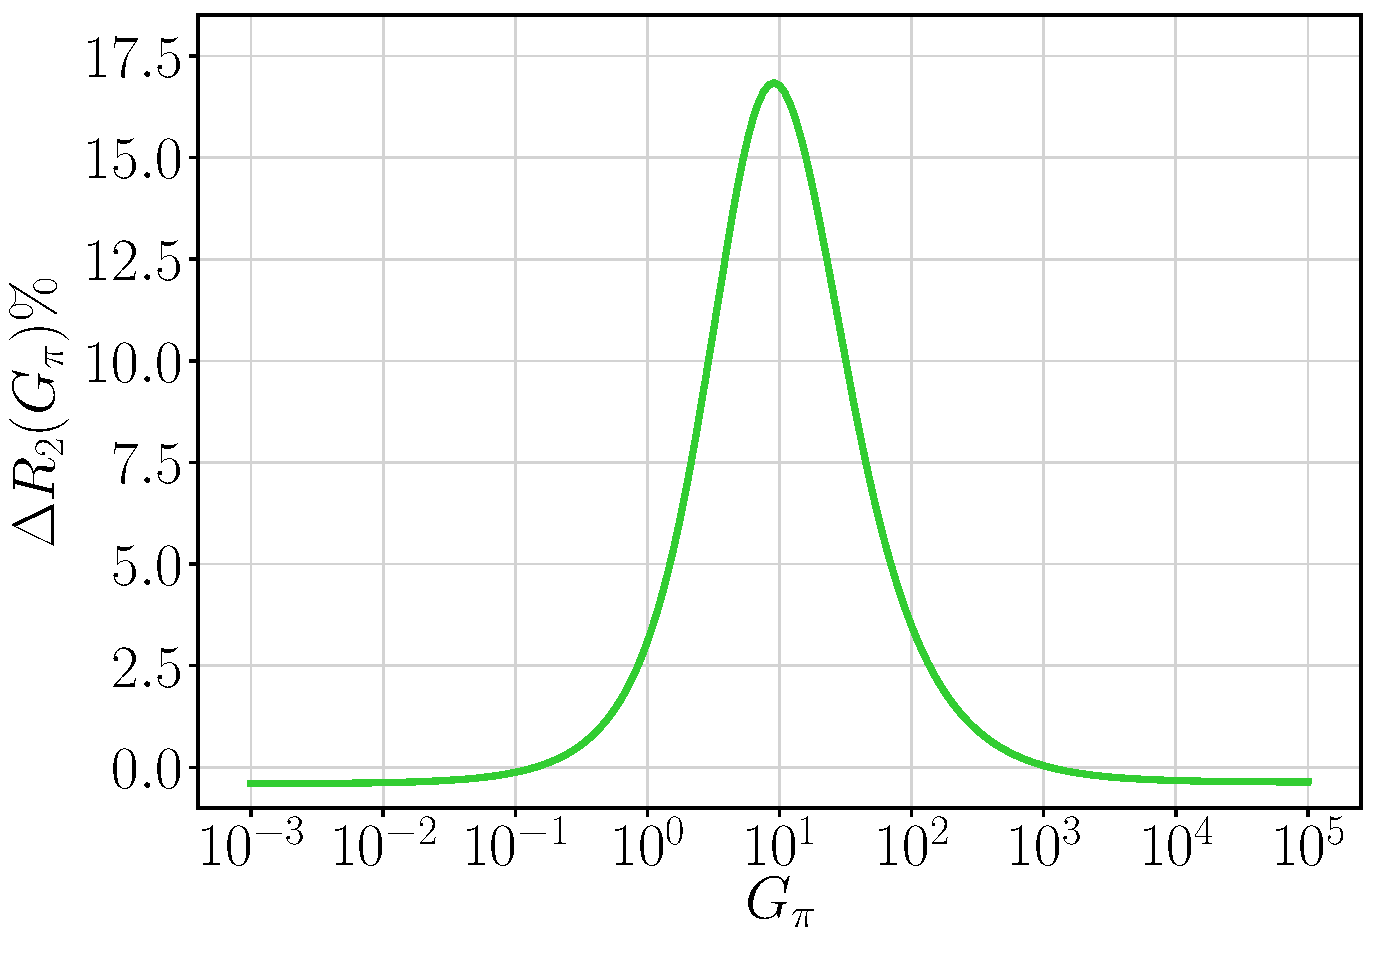
\includegraphics[width=.8\linewidth]{Figures/chapter05/G2-logerr}
		\end{minipage} \\[-1em]
		\begin{center}
			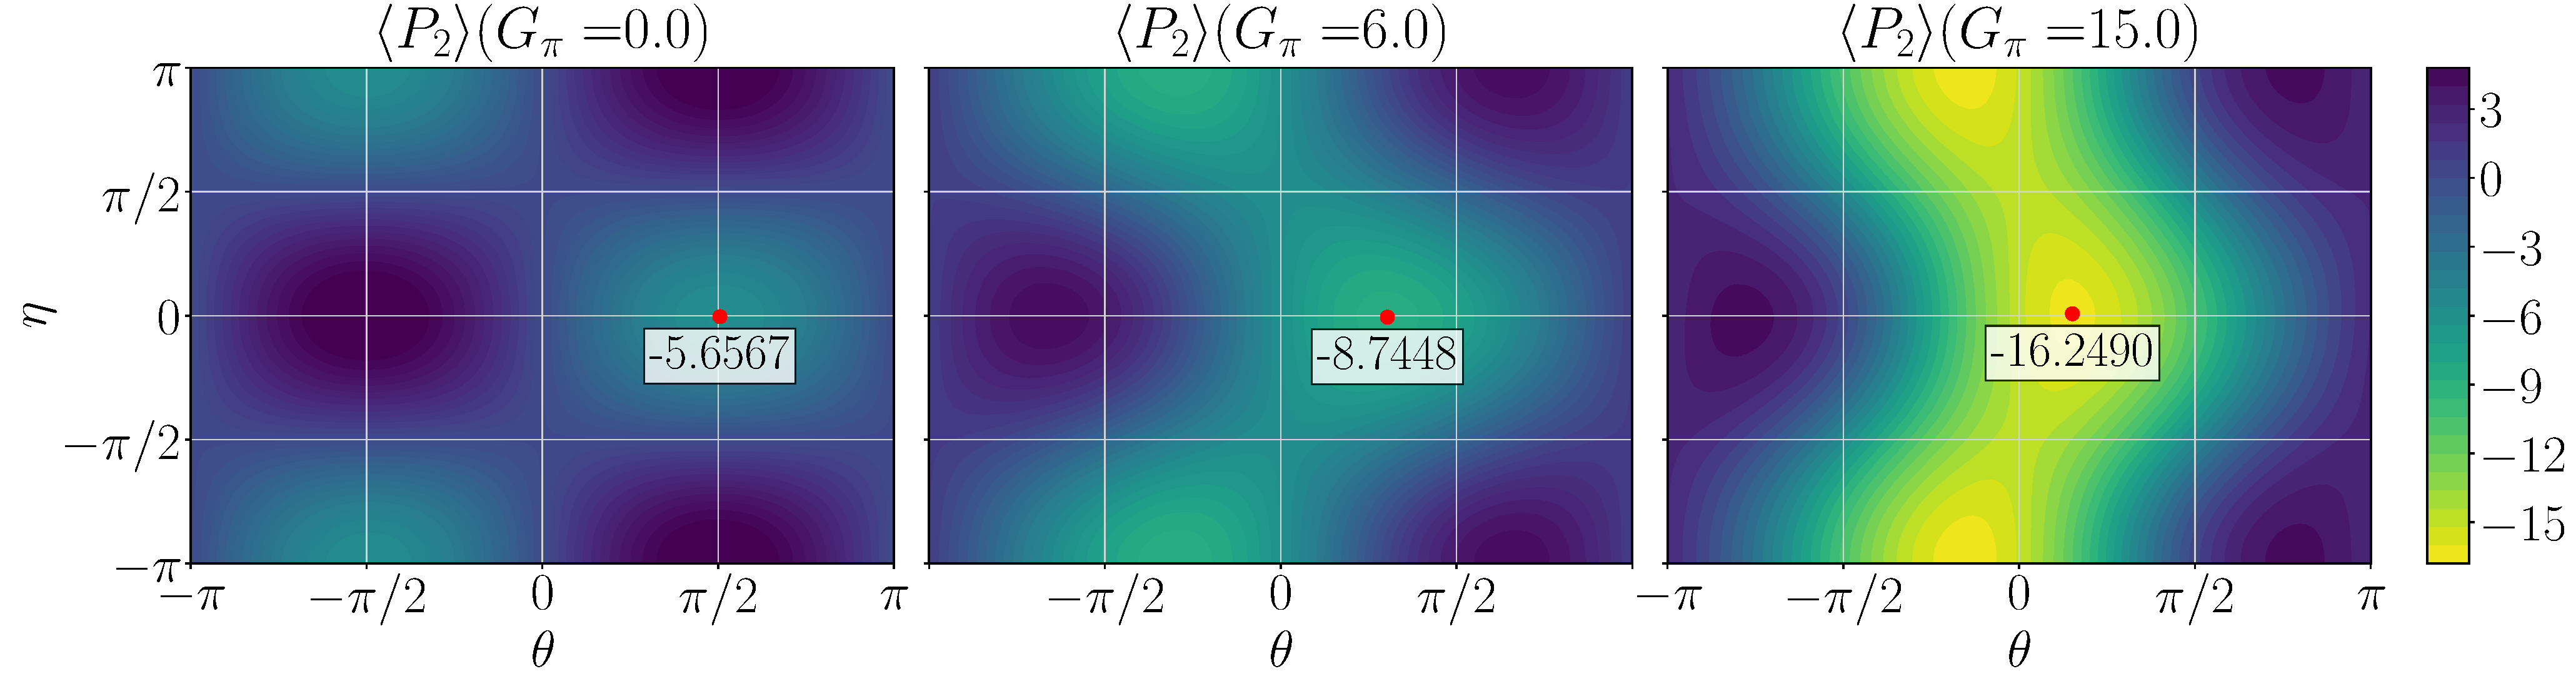
\includegraphics[width=.7\paperwidth]{Figures/chapter05/P2-tri-contour}
		\end{center}
		% \caption{Percentual error of the ground state energy results obtained from our quantum simulation with respect to the analytical solution and for different values of the coupling constant. (Left) Linear scale. (Right) Logarithmic scale.}
	\end{figure}
	\vspace{-2em}

\end{frame}
